\chapter{Contact-Rich Manipulation Planning using Quasi-static Models} \label{chapter:contact_rich_planning}
\section{Introduction}
In Chapter 2, we have developed the CQDC dynamics and prposed computational methods to obtain local linear models of its smooth surrogate. These tools are not specific to any algorithm: they can improve the performance of most iterative planning algorithms that rely on local approximations. 

We start the section on contact-rich planning with iterative MPC (iMPC) \cite{bundledgradients}, a variant of trajectory optimization, that uses the CQDC dynamics to enforce contact dynamics constraints and compute smoothed gradients. In addition to demonstrating the utility of the proposed CQDC dynamics, we also introduce iMPC as a handy refinement tool for trajectories generated by a sampling-based motion planner (SBMP). Such trajectories are well-known for making inefficient and meandering ``dances'' before arriving at the goal. 

However, we have argued that the success of contact-rich planning depends on both smoothing and global search. Planning based on local optimization, including trajectory optimization with smoothed contact dynamics, generally results in non-convex optimization problems where the quality of different local minima can be a make-or-break factor. Solving such problems requires non-trivial initialization and cost tuning \cite{onol2020tuning}, both of which can be highly problem specific and notoriously hard to debug. This motivates us to search further for a more global approach.

In robotics, SBMP algorithms such as the Rapidly-Exploring Random Tree (RRT) \cite{lavalle1998rapidly} are widely used for global search problems, including those with kinodynamic constraints \cite{karaman2010optimal}. However, the success of such planners has rarely extended to contact-rich settings. We find that while optimization-based methods for planning through contact have employed smoothing schemes, all existing SBMP methods for contact planning explicitly consider modes instead of smoothing them \cite{cheng2021contact,wu2020r3t,chen2021trajectotree,motioncones,terry}, as SBMP methods do not inherently require local characterizations of dynamics (i.e. gradients). Yet, previous works have shown that such local models are highly relevant for designing more efficient distance metrics during the nearest neighbor queries that respects dynamic reachability \cite{shkolnik2009reachability,wu2020r3t,haddad2021anytime}.

In this chpater, we fill in this gap by combining contact mode abstraction via smoothing, and the global search capabilities of RRT. We enable RRT to explore efficiently through contact constraints by utilizing a novel distance metric based on the local smoothed linearizations of CQDC dynamics (Sec.\ref{sec:mahalanobis}). In addition, we further propose an efficient extension step by computing actions that expand the tree to new parts of the state space using the local linearizations (Sec.\ref{sec:rrt_for_contact}). With a variety of contact-rich tasks inspired by \cite{rajeswaran2018learning} that involve both intrinsic and extrinsic dexterity \cite{extrinsic}, we show that combining smoothing with RRT achieves tractable global motion planning for highly contact-rich manipulation (Sec.\ref{sec:rrt_results}); and that the planned trajectories can transfer to high-fidelity second-order simulations or even robot hardware. To the best of our knowledge, our work appears to be the first to successfully combine SBMP with contact mode smoothing.

\section{Trajectory Optimization through Contact \label{sec:traj_opt}}
\noindent 
In this section, we demonstrate the efficacy of smoothed CQDC dynamics on trajectory optimization for systems with contacts.
Although smoothing of hard contact constraints has been widely utilized to improve convergence \cite{posa2014direct, howell2022dojo, howell2022trajectory}, existing methods still struggle with complex problems such as dexterous manipulation. In particular, the quality of solutions can be very sensitive to initial guesses \cite{onol2020tuning}.
In this context, we show that a variant of trajectory optimization, with the help of smoothed CQDC dynamics and only a trivial initial guess, can perform well even on dexterous manipulation tasks.

\subsection{Iterative MPC with Smoothing \label{sec:iMPC}}
The variant of trajectory optimization algorithm used in this section, which we call iterative MPC (iMPC), is an iLQR-inspired algorithm proposed in \cite{bundledgradients}. We briefly summarize iMPC here for completeness, and illustrate how smoothing can be easily integrated into iMPC.

Consider the problem of finding an optimal sequence of inputs to track some desired state trajectory $\{x^d_t\}_{t=0}^T$. We need an initial guess for the nominal input trajectory $\{\bar{u}_t\}^{T-1}_{t=0}$, from which the nominal state trajectory $\{\bar{x}_t\}^T_{t=0}$ can be obtained by rolling out $\{\bar{u}_t\}^{T-1}_{t=0}$ from the initial state $x_0$. For every time $t$ (i.e. in a time-varying manner), we can create a locally linear model that approximates the dynamics, with model parameters $\{\mathbf{A}_t,\mathbf{B}_t,c_t\}_{t=0}^{T-1}$ \eqref{eq:linearization}. Then, finding the optimal $\{\bar{u}_t\}^{T-1}_{t=0}$, subject to the locally linear model of the dynamics, can be written as a QP. We present the MPC variant of this problem that receives the initial state $\bar{x}_j$ at time $t=j$ and computes the optimal action for the remaining time steps,
\begin{subequations}
\label{eq:trajopt}
\begin{align}
\textbf{MPC}(\bar{x}_j) & = u^\star_j, \text{where}\\
\{x_t^\star\}_{t=j}^T, \{u_t^\star\}_{t=j}^{T-1}
=\underset{\{x_t\}_{t=j}^T, \{u_t\}_{t=j}^{T-1}}{\text{argmin}} & \norm{x_T-x_T^d}_{\mathbf{Q}_T}^2 + \sum^{T-1}_{t=j} \left(\|x_t - x^d_t\|^2_{\mathbf{Q}_t} + \|u_t\|^2_{\mathbf{R}_t}\right)\\
\text{s.t.}\;\; & x_{t+1} = \mathbf{A}_t(x_t-\bar{x}_t) + \mathbf{B}_t(u_t - \bar{u}_t) + c_t,\\
& \mathbf{C}^x_t x_t\leq d^x_t,\; \mathbf{C}^u_t u_t \leq d^u_t, \; \forall t\in\{j \cdots T-1\},\\
& x_j = \bar{x}_j.
\label{eq:trajopt:x_u_constraints}
\end{align}
\end{subequations}

Here, $\{\mathbf{Q}_t,\mathbf{R}_t\}$ are the quadratic weights for state and input, respectively; $\mathbf{Q}_T$ is the weight on the terminal state; $\{\mathbf{C}^x_t,d^x_t\}$ and $\{\mathbf{C}^u_t,d^u_t\}$ are inequality parameters on the state and input, respectively. The linear constraints \eqref{eq:trajopt:x_u_constraints} can enforce, for instance, joint and actuation limits.

The iMPC algorithm is summarized in Alg. \ref{alg:impc}. 
In every outer iteration (body of the $\mathtt{while}$ loop starting at Line \ref{alg:impc:while}), iMPC solves truncated versions of \eqref{eq:trajopt} for $T - 1$ times. Specifically, at inner iteration $j$ (body of the $\mathtt{for}$ loop starting at Line \ref{alg:impc:for}), we solve MPC \eqref{eq:trajopt} for the sub-problem starting at $t=j$ (Line \ref{alg:impc:mpc}), and apply $u_j^\star$ from the solution to update $\bar{x}_{j+1}$ (Line \ref{alg:impc:update_x}). In every inner iteration, we also enforce a trust region by using \eqref{eq:trajopt:x_u_constraints} to constrain $x_t$ and $u_t$ to stay close to $\bar{x}_t$ and $\bar{u}_t$, respectively.

\begin{algorithm}
\caption{\textbf{iMPC}}\label{alg:impc}
\textbf{Input:} Initial state $x_0$, input trajectory guess $\{\bar{u}_t\}_{t=0}^{T-1}$\;
\textbf{Output:} Optimized input trajectory $\{\bar{u}_t\}_{t=0}^{T-1}$ \;
$\{\bar{x}_t\}_{t=0}^T\leftarrow$ Rollout $f$ from $x_0$ with$\{\bar{u}_t\}_{t=0}^{T-1}$\;
\While {\textrm{not converged}}{ \label{alg:impc:while}
    Compute system matrices $\{\mathbf{A}_t,\mathbf{B}_t,c_t\}_{t=0}^{T-1}$\;
    \For {$0\leq j < T$} { \label{alg:impc:for}
        $\bar{u}_j \leftarrow \mathbf{MPC}(\bar{x}_j)$ \label{alg:impc:mpc}\; 
        $\bar{x}_{j+1} \leftarrow f(\bar{x}_j,\bar{u}_j)$ \label{alg:impc:update_x}\;
    }
}
\algorithmicreturn $\; \{\bar{u}_t\}_{t=0}^{T-1}$
\end{algorithm}

To apply smoothing to iMPC, we substitute the linearizations of smooth surrogates $\{\mathbf{A}_{t,\rho},\mathbf{B}_{t,\rho},c_{t,\rho}\}^{T-1}_{t=0}$ \eqref{eq:ABc_rho} for the first-order Taylor expansions $\{\mathbf{A}_t,\mathbf{B}_t,c_t\}_{t=0}^{T-1}$ \eqref{eq:linearization}. After every outer iteration, we also reduce the variance of $\rho$ (this can be done for analytic smoothing by increasing the log barrier weight $\kappa$), allowing the smooth surrogates $f_\rho$ to converge to the true CQDC dynamics $f$.

\begin{figure*}
\centering
\subfloat[\code{PlanarPushing}.]{
	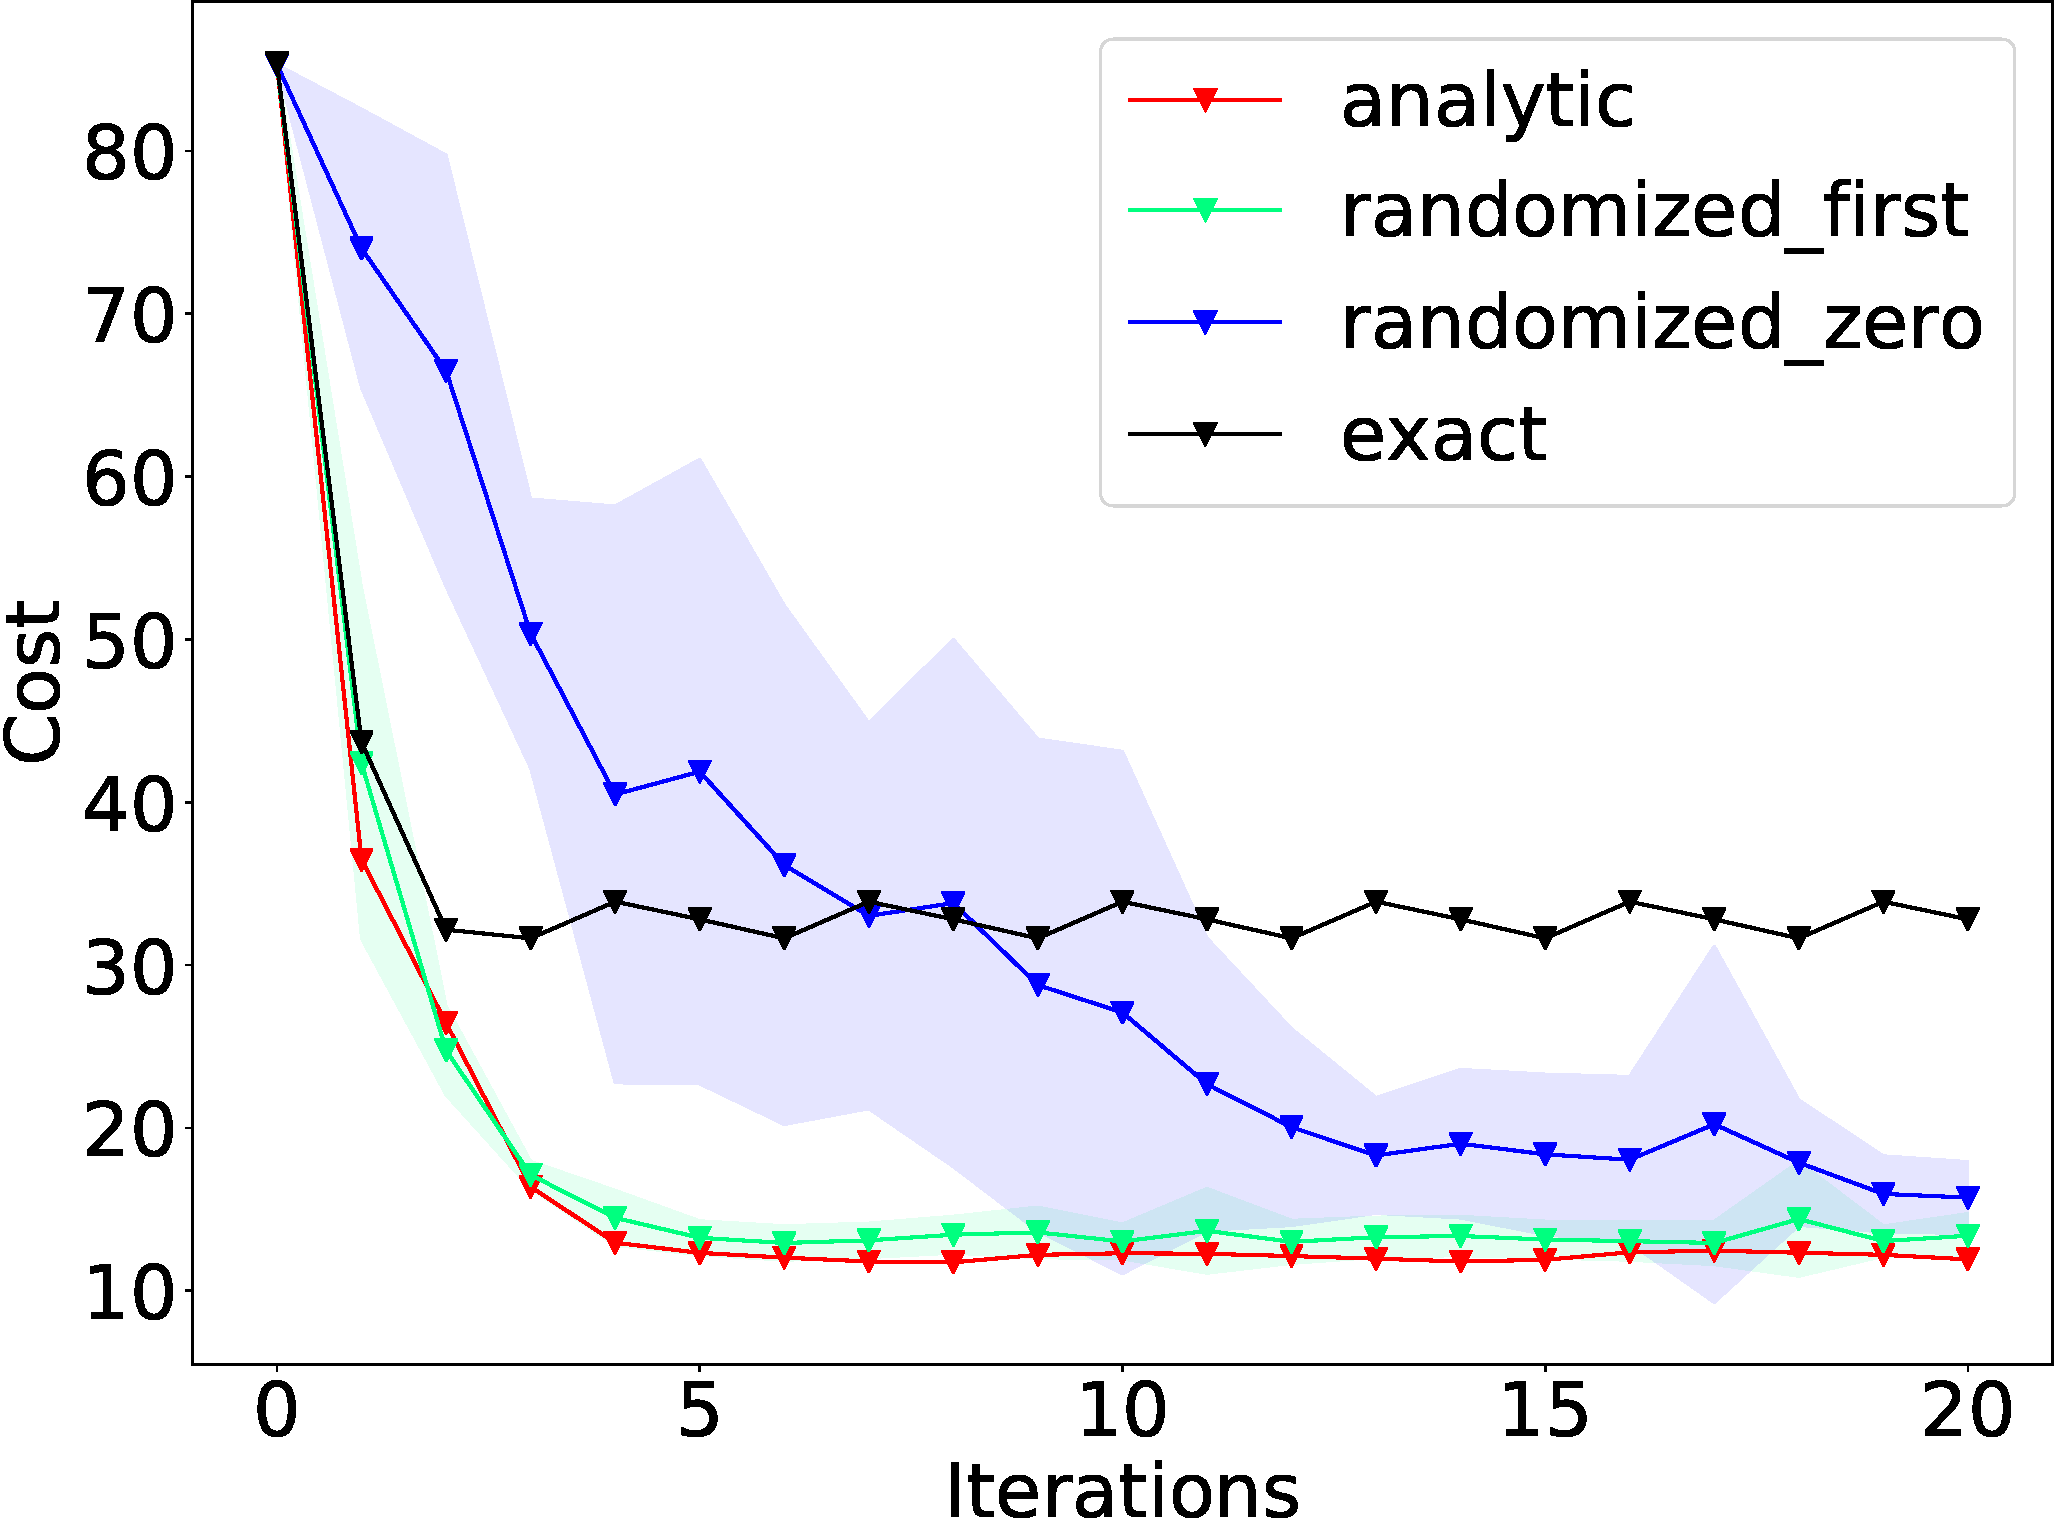
\includegraphics[width=0.32\linewidth]{figures/03_contact_rich_planning/trajopt_results/planar_pushing.pdf}
}
\subfloat[\code{PlanarHand} Re-orientation.]{
	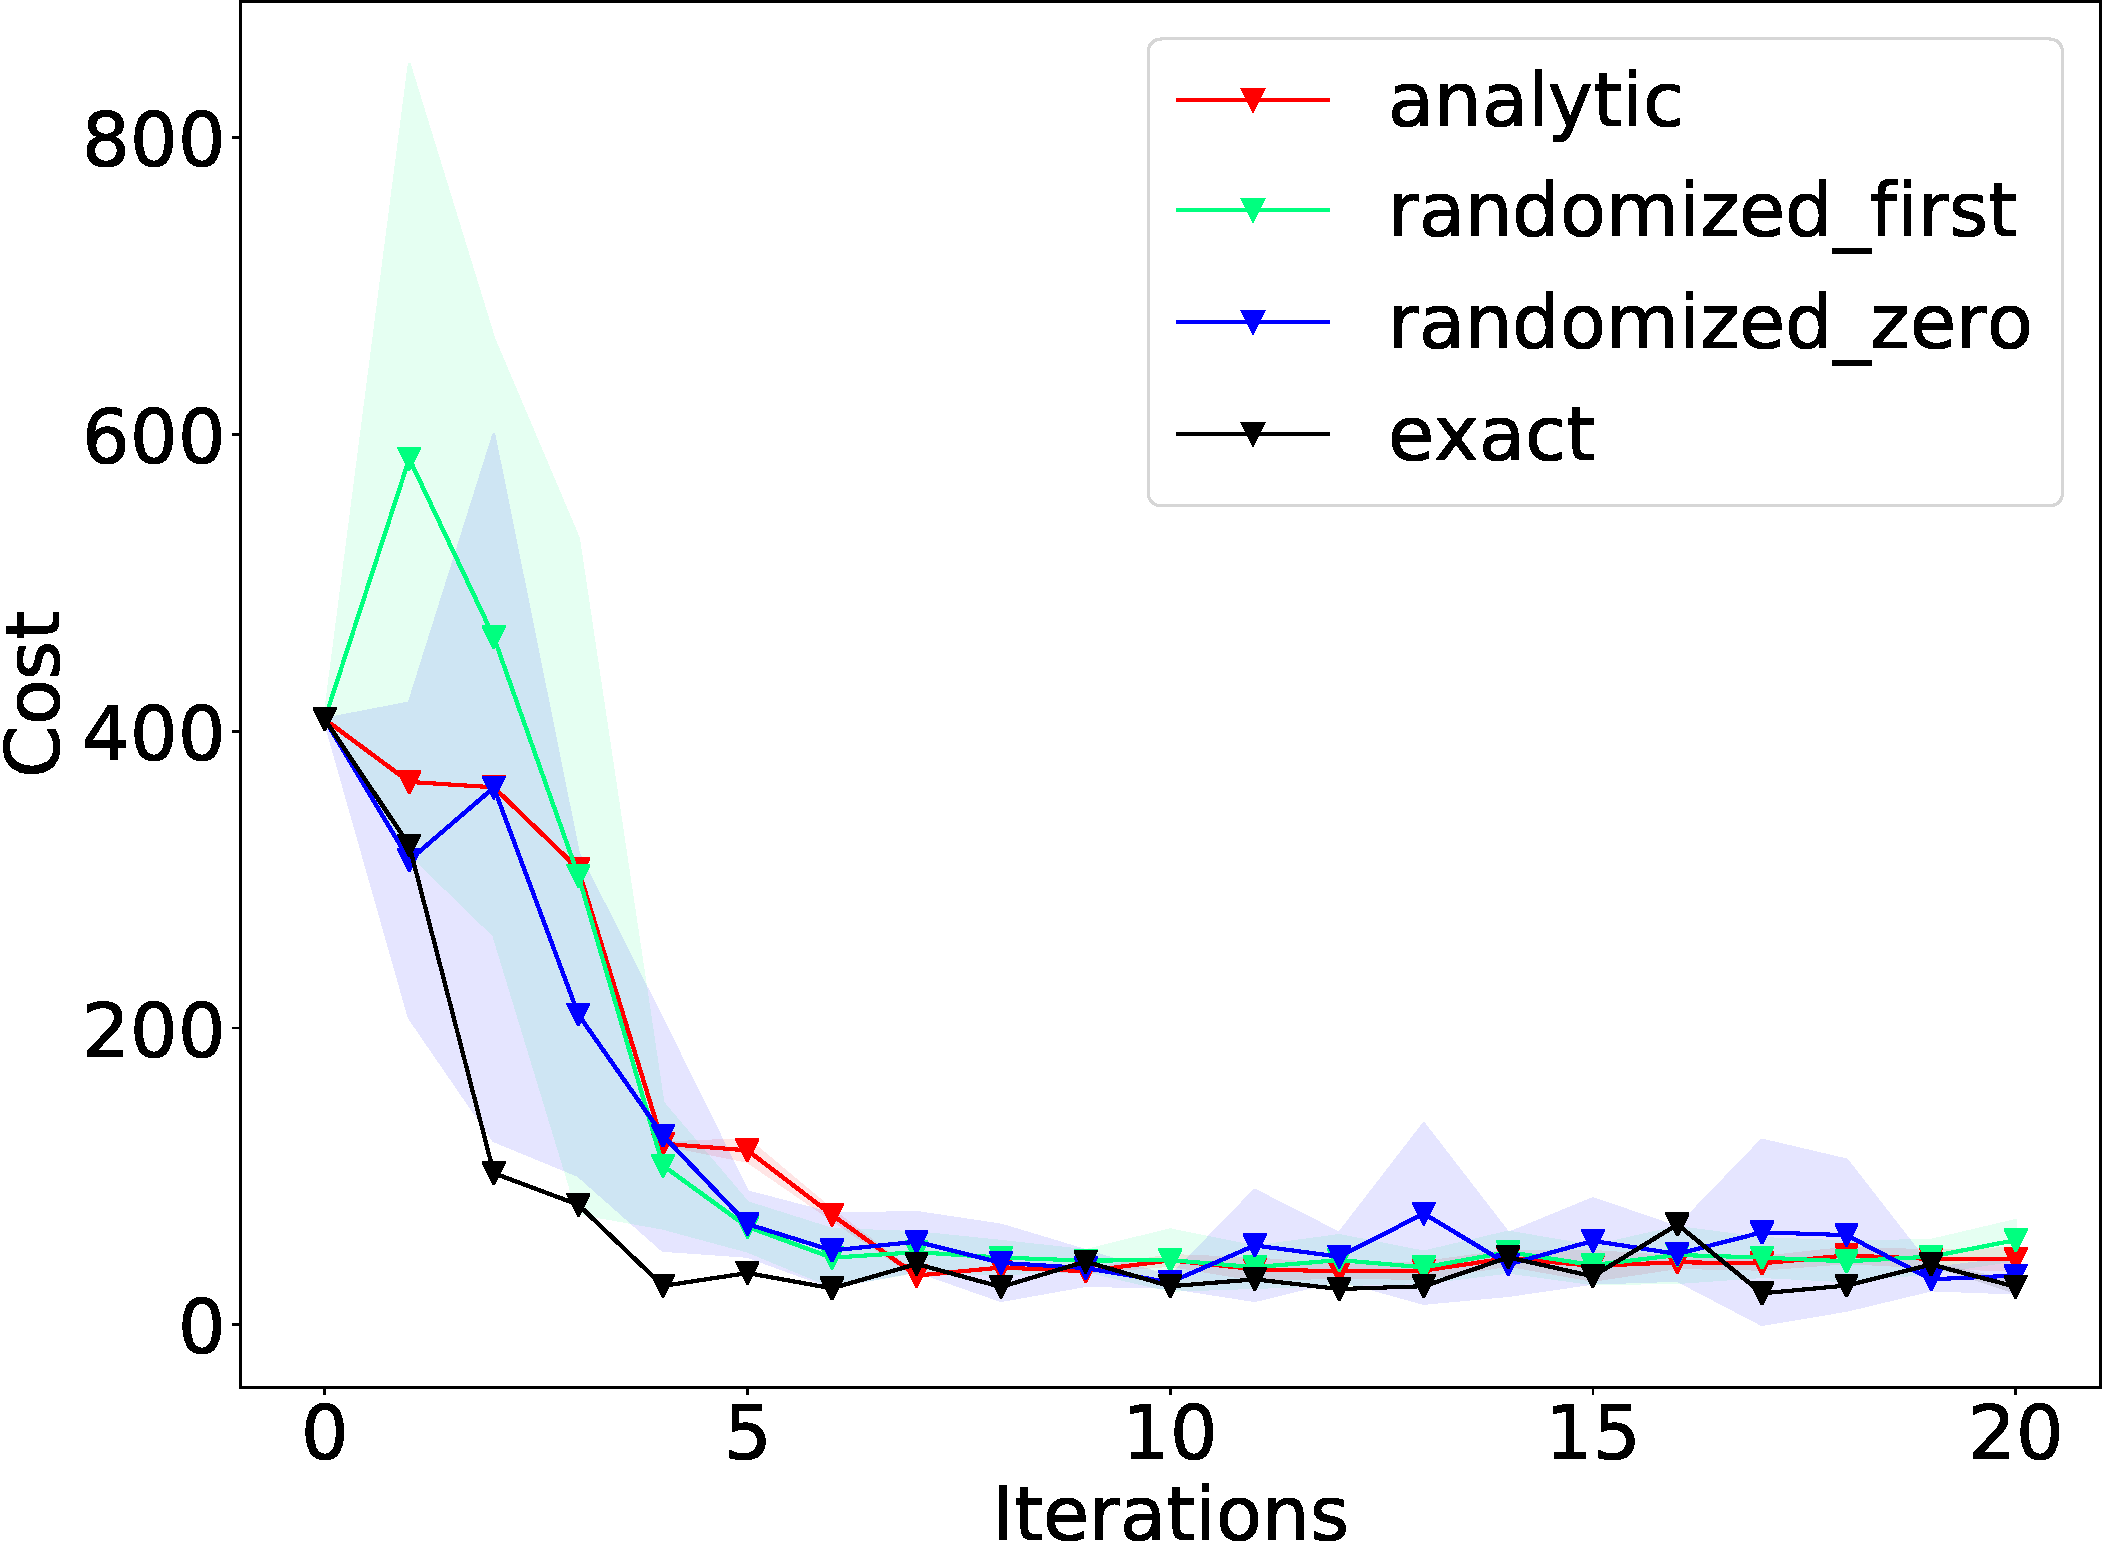
\includegraphics[width=0.32\linewidth]{figures/03_contact_rich_planning/trajopt_results/planar_hand.pdf}
}
\subfloat[\code{AllegroHand} Rotation.]{
	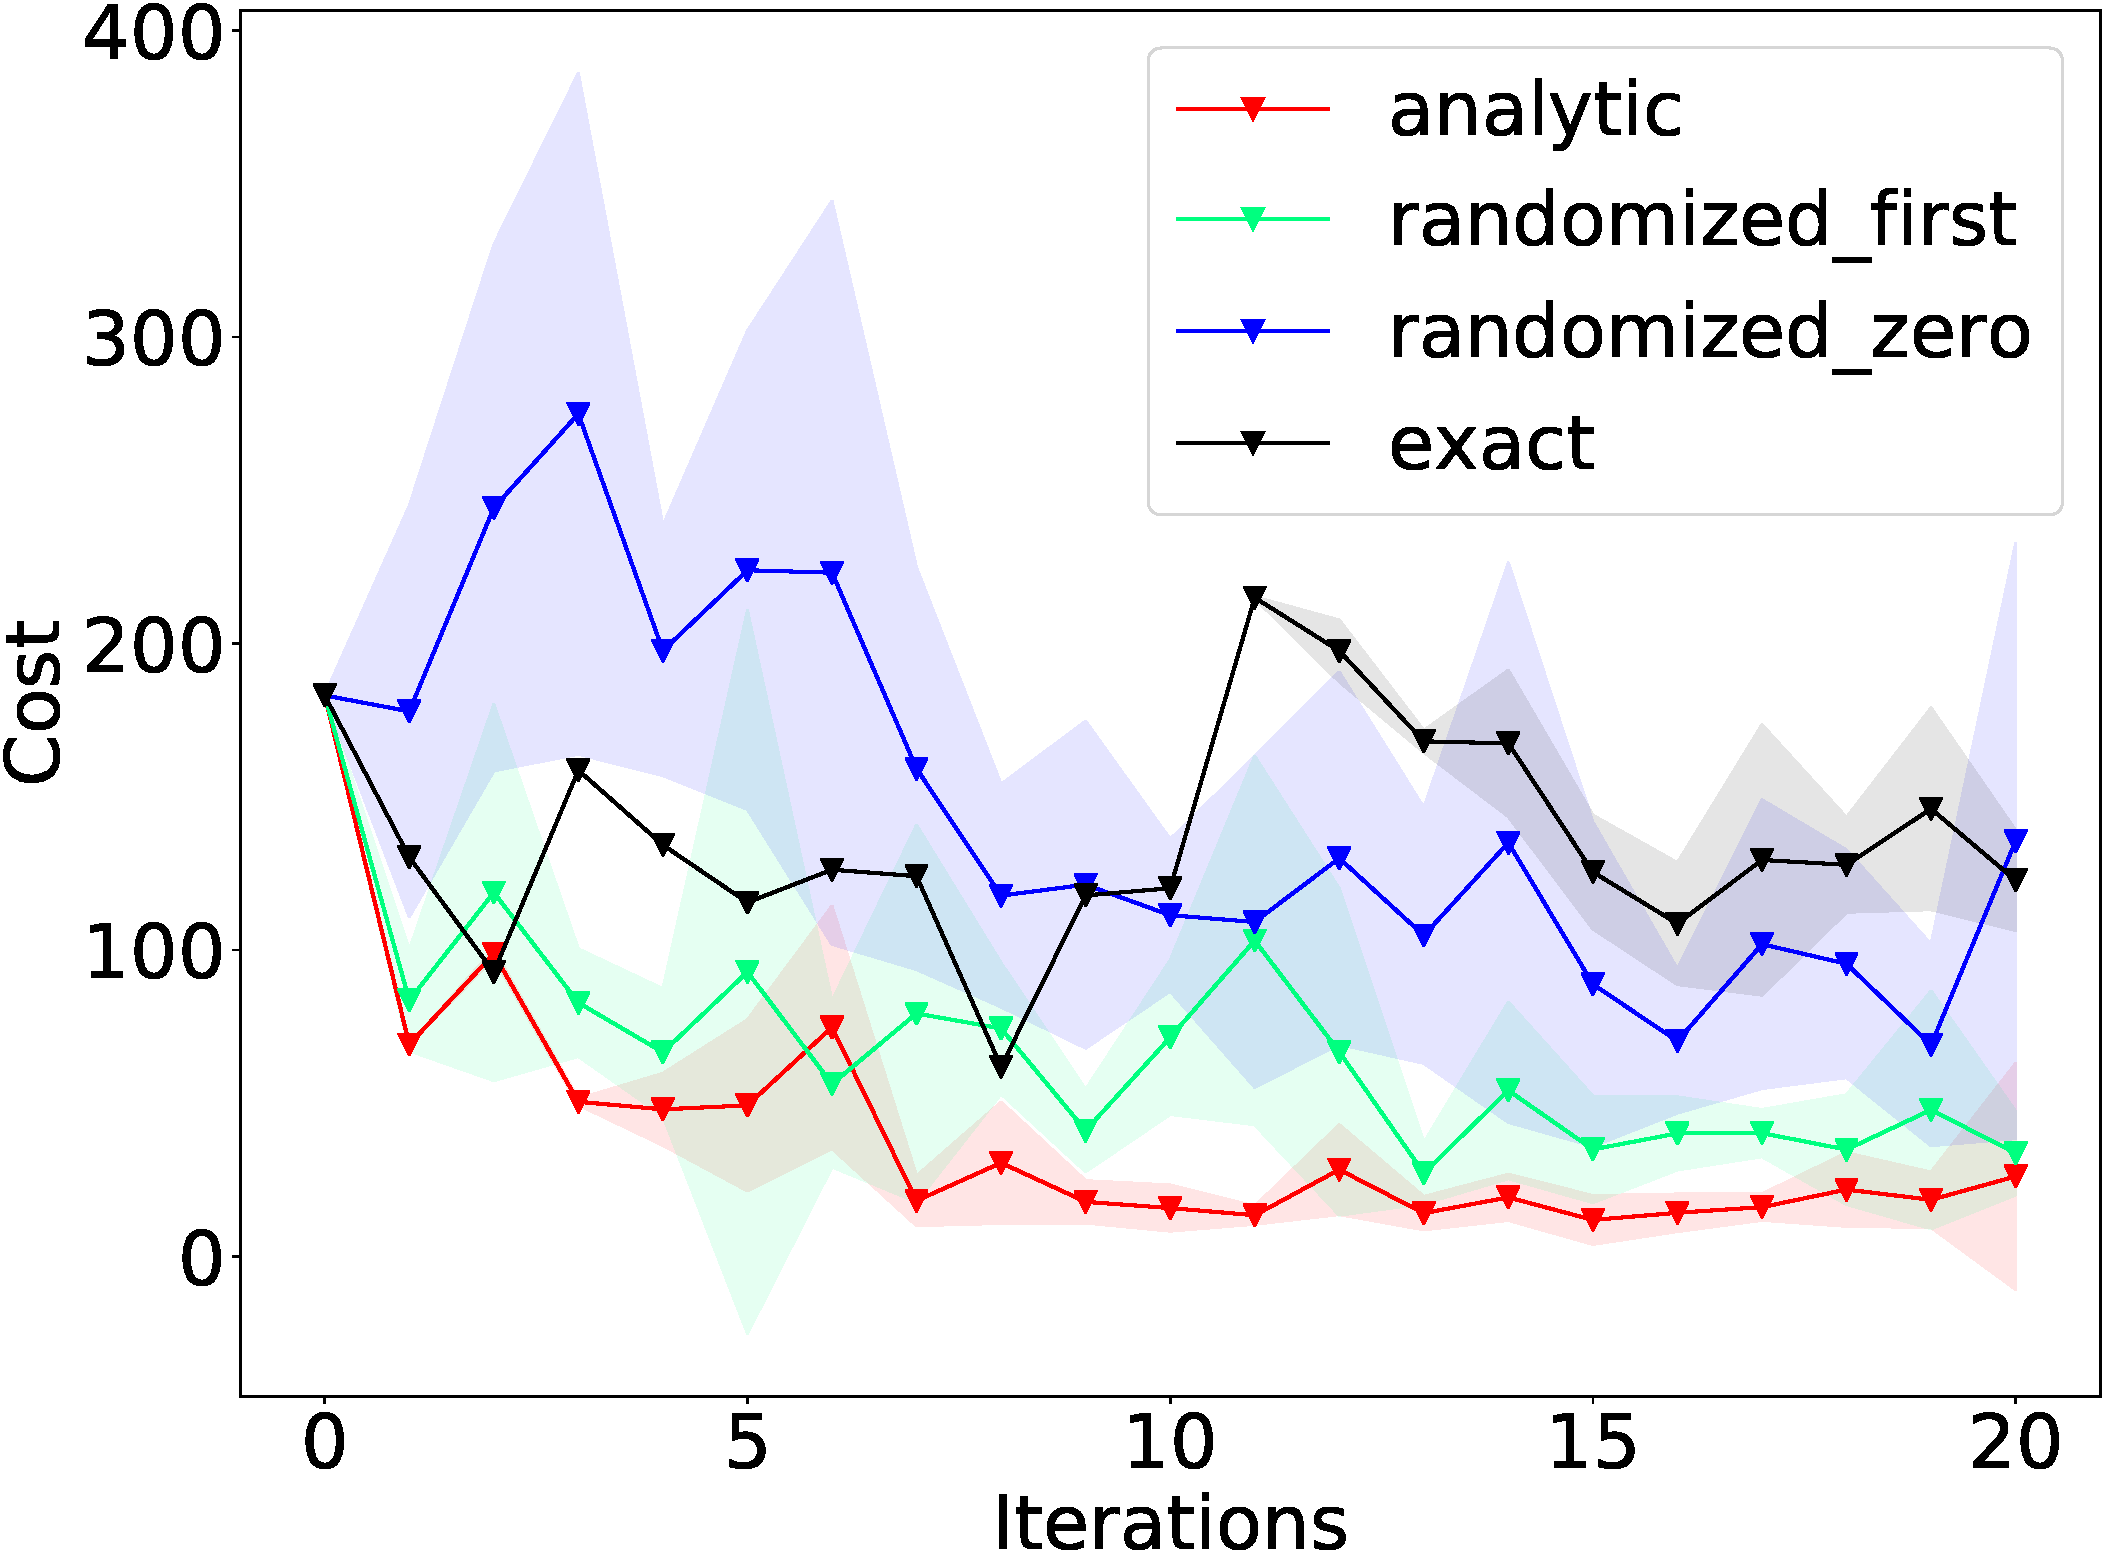
\includegraphics[width=0.32\linewidth]{figures/03_contact_rich_planning/trajopt_results/allegro_hand.pdf}
}
\caption{Performance of iMPC with different smoothing schemes: analytic, randomized (first-order), randomized zero-order, and exact (no smoothing). For each method, the solid line represents the mean over five runs, and the shaded region represents the standard deviation. }
\label{fig:trajoptperformance}
\end{figure*}

\subsection{Experiment Setup}\label{sec:trajopt_setup}
\subsubsection{Systems Description \label{sec:trajopt_setup:systems}}
We test iMPC with different smoothing schemes on two planar systems from \cite{bundledgradients} and a 3D system for in-hand rotation. We describe our systems below, and their visualization can be seen in Fig. \ref{fig:rrtperformance}. The three tuple after the name of each system indicates $(\nU, \nA, \nCG)$, where $\nU$ is the number of unactuated DOFs, $\nA$ the number of actuated DOFs, and $\nCG$ the number of collision geometries.

\begin{enumerate}
\item {\bf Planar Pushing, (3,2,2)}.  A classical example of nonprehensile manipulation \cite{lynch1996stable}. The goal is specified as some 2D configuration of the box.
\item {\bf Planar Hand Reorientation, (3,4,13)}.  We use a planar hand with two fingers, each with two DOFs. The goal is to change the position and orientation of the ball in a 2D plane.
% , the 2D robot pushes the object to desired position and orientation. 
\item {\bf Allegro In-Hand Rotation, (6,16,20)}.  3D In-hand rotation of the ball with the full model of the allegro hand \cite{huang2020efficient}. The goal is specified as a rotated configuration of the ball.
\end{enumerate}

\subsubsection{Initialization}
As mentioned in Sec. \ref{sec:iMPC}, given an initial state $x_0$, we need to initialize the nominal input trajectory $\{\bar{u}_t\}^{T-1}_{t=0}$, where $\bar{u}_t$ is the commanded positions of the robots at step $t$ under the CQDC dynamics. Empirically, we find that good convergence can be achieved with a constant initialization, i.e. $\bar{u}_0 = \bar{u}_1 = \dots \bar{u}_{T-1}$. Although this initialization is still prone to local minima, it is surprisingly effective when the solution can be found without global search.

For the numerical experiments in this section, we need a $\bar{u}_0$ that makes contact with the object. Otherwise the baseline which does not use smoothing would have zero gradients and make no progress at all. 

In contrast, for iMPC with smoothing, it is sufficient to set $\bar{u}_0 = q^\mathrm{a}_0$, as long as $q^\mathrm{a}_0$ is not ``too far away'' from making contact with the objects (the reason is explained in Example \ref{ex:planarhandreachableset}). In many practical problems, the object's initial configuration $q^\mathrm{u}_0$ is fixed, but we are free to choose the initial robot configuration $q^\mathrm{a}_0$. In this case, we can simply calculate a $q^\mathrm{a}_0$ that is ``close'' to making contact using, for example, methods that compute grasps \cite{murray2017mathematical}. 

\subsubsection{Hardware \& Implementation Details}
The numerical experiments are run on a desktop with one AMD Threadripper 2950 CPU (16 cores, 32 threads) and 32GB of RAM. The code for iMPC using different smoothing schemes is identical except for the computation of the linearizations. For analytic smoothing and the baseline, we solve respectively the smoothed \eqref{eq:q_dynamics_log} and original \eqref{eq:q_dynamic_socp} dynamics once and then apply the chain rule to get the linearization. For first-order randomized smoothing, we solve the original dynamics \eqref{eq:q_dynamic_socp} and apply the chain rule for 100 samples ($N=100$), which is parallelized on all available threads, and then average the gradients of the samples. Zeroth-order randomized smoothing simply requires parallel evaluation of the dynamics.


\begin{figure}[t]
\centering
\subfloat[Initial configurations and goals. Each system is shown in its initial configuration $q_0$. The thicker frame denotes the goal while the thinner frame denotes the initial configuration of the object.]{
	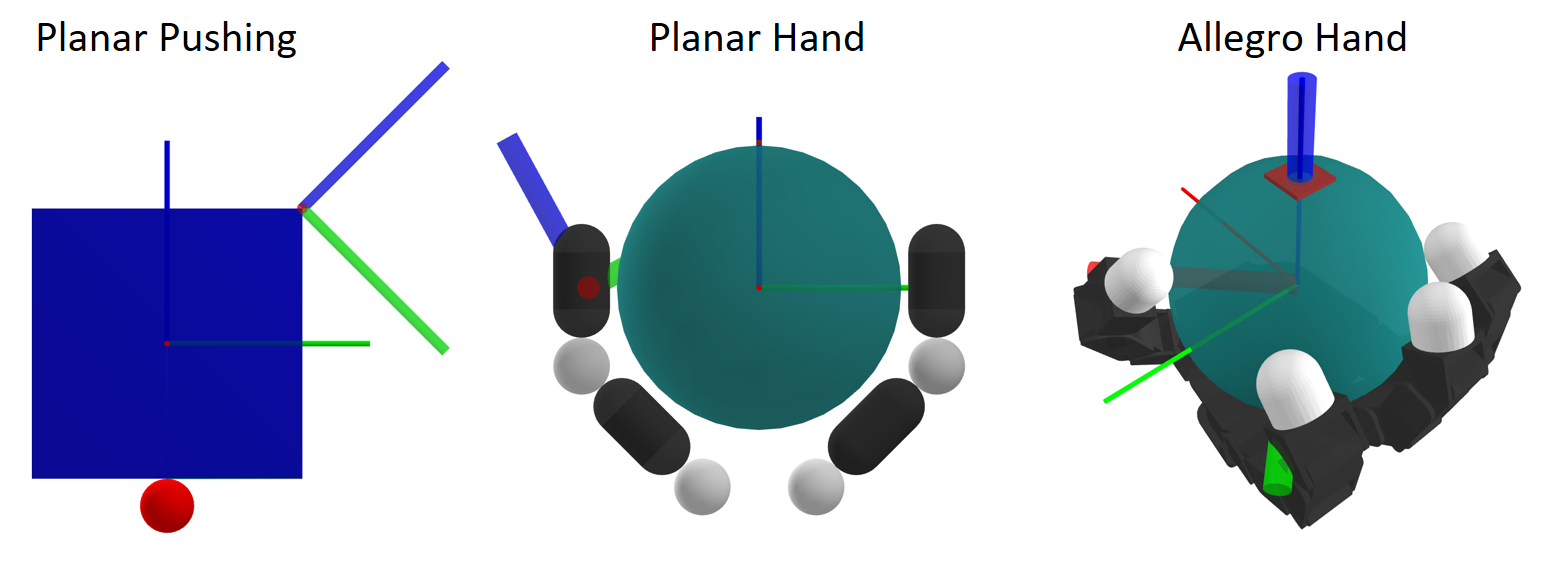
\includegraphics[width=0.80\textwidth]{figures/03_contact_rich_planning/trajopt_tasks.png}
	\label{fig:trajopttasks}
}\\
\subfloat[Final object configuration achieved by the best runs within each of the four methods. Pink shaded denotes the goal configuration for the first two examples, while the goal configuration in the last example is marked by the pink line protruding out of the object. Colors correspond to the plots in Fig. \ref{fig:trajoptperformance}.]{
    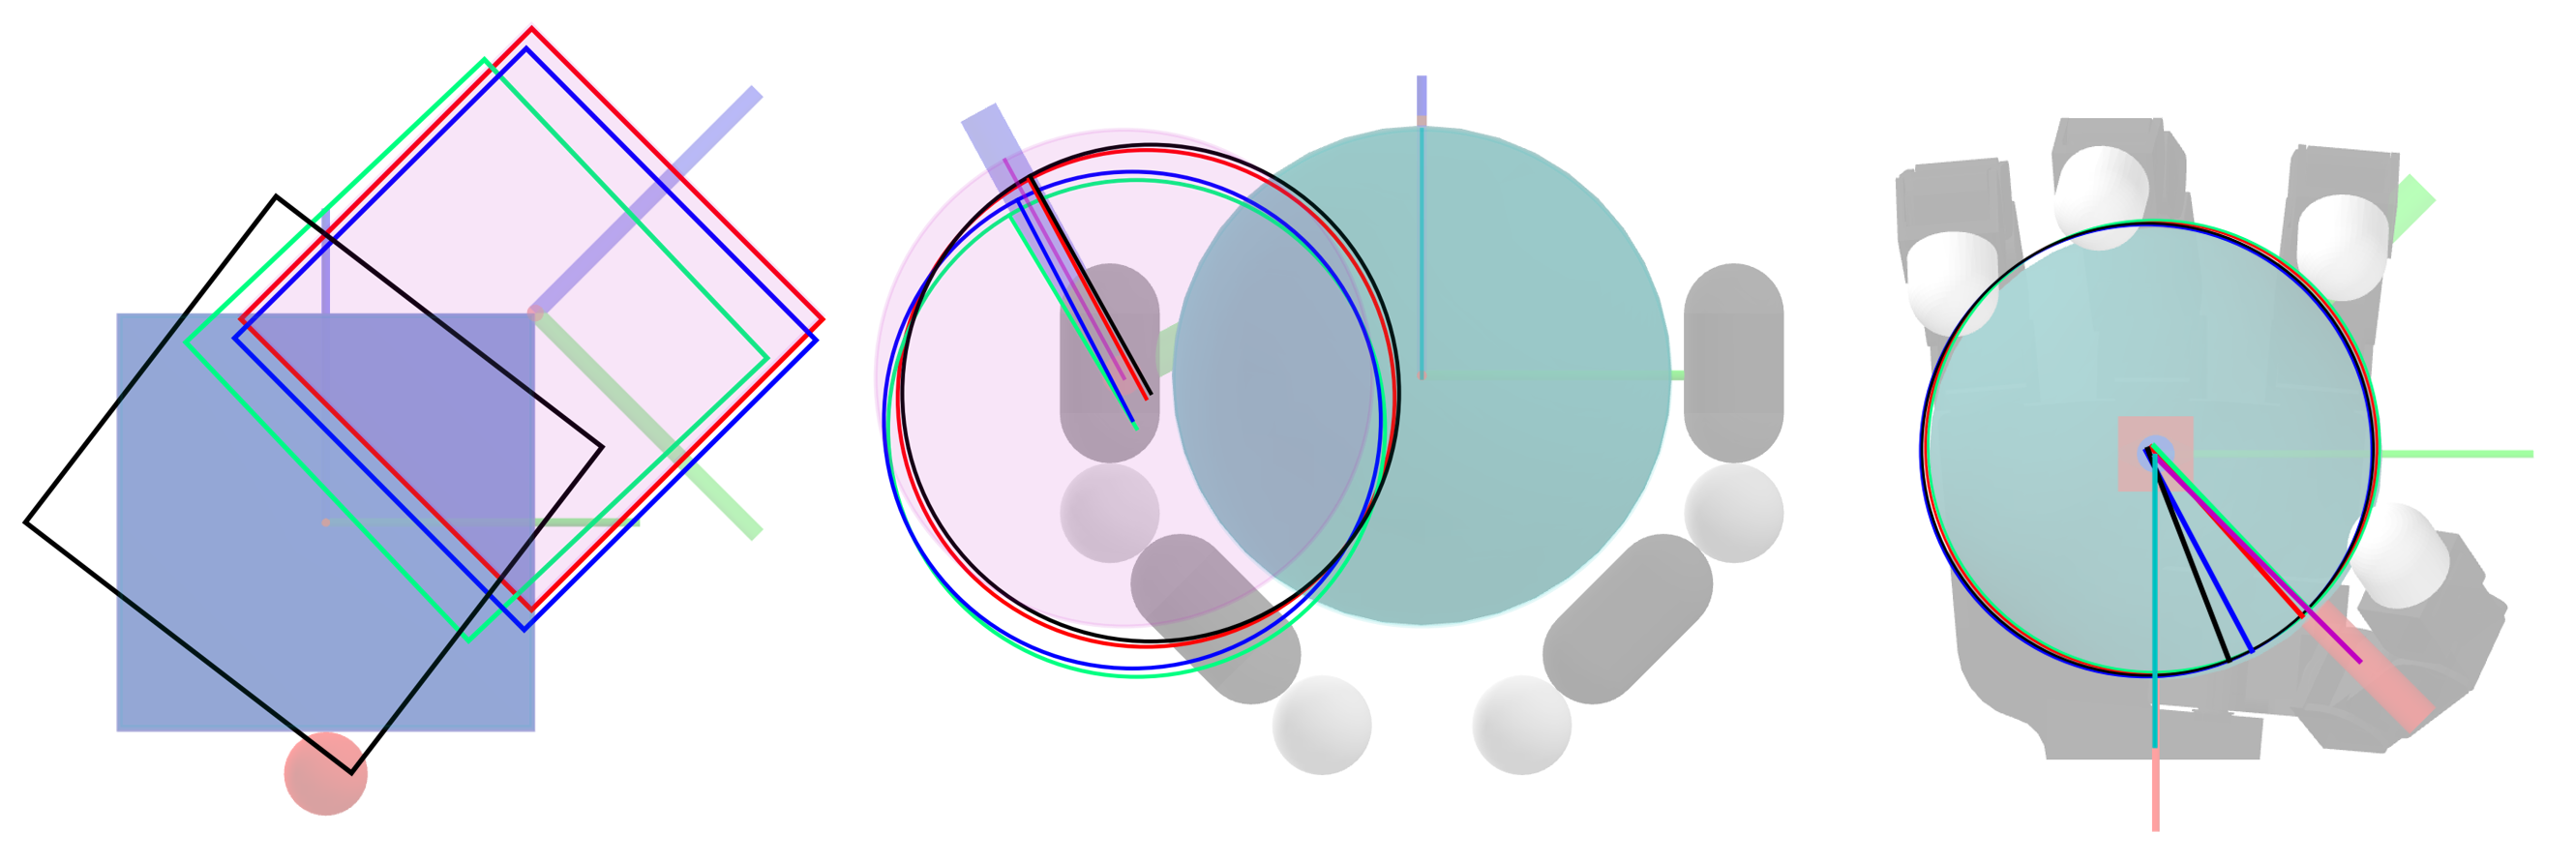
\includegraphics[width = 0.80\textwidth]{figures/03_contact_rich_planning/trajopt_results_vis.png}
    \label{fig:trajoptvis}
}
\caption{Tasks and results for the trajectory optimization case study.}
\label{fig:trajopt}
\end{figure}

\begin{table}[thpb] \label{tab:trajoptresults}
\centering
\begin{tabular}{|| c | r | r | r | r | r | r |} 
 \hline
 Problem & \multicolumn{2}{||c||}{PlanarPushing} & \multicolumn{2}{||c||}{PlanarHand} & \multicolumn{2}{||c||}{AllegroHand}  \\\hline
 Method & Cost & Time(s) & Cost & Time(s) & Cost & Time(s) \\ \hline\hline

    A.        & 11.74 & 2.17  & 26.55 &  5.20  & \bf{5.78} & 19.59  \\
    RF.       & \bf{11.73} & 4.64 & \bf{17.8}7 & 23.09 & 8.42 & 40.07 \\
    RZ.      & 12.86 & 4.61 & 18.29 & 11.93 & 28.21 & 34.05 \\
    E.            & 31.64 & 1.88 & 18.49 & 5.91 & 44.68 & 12.92 \\\hline
\end{tabular}
\caption{Minimum cost and running time achieved by different methods. All methods are ran for $10$ iterations across 5 trials. The methods names are abbreviations from the legend of Fig. \ref{fig:trajoptperformance}.}
\label{table:trajoptresults}
\vspace{-0.2cm}
\end{table}

%we note that we always initialize the system to be in a contacting configuration, as otherwise the gradient without smoothing is always zero in a non-contacting configuration. Consequently, algorithms that rely on exact linearization simply makes no progress. Though we initialize this way to give exact linearization an advantage, we note that the ability to converge from a non-contacting configuration is also a strength of using smooth surrogates.

\subsection{Results \& Discussion}
In Fig. \ref{fig:trajoptperformance}, we plot the performance of iMPC with a baseline that does not use smoothing, and the three different smoothing schemes in Sec. \ref{sec:smoothdynamics}, namely analytic, randomized first-order, and randomized zeroth-order. We also summarize the running time of each method, as well as the minimum cost achieved across the iterations, in Table \ref{table:trajoptresults}. Illustrations of the tasks and the results achieved by different methods are shown in Fig. \ref{fig:trajopt}. We interpret the results and discuss the relevant findings in this section. 
\subsubsection{Exact vs. Smoothing} For \code{PlanarPushing} and \code{AllegroRotation}, the various smoothing schemes achieve much lower costs than using exact gradients. However, for \code{PlanarHand}, using the exact linearization is performant as well. This difference may be explained by the observation that the planar hand example does not go through many mode changes, while the planar pusher and the allegro hand require several mode changes to converge to the locally optimal trajectory. 

\subsubsection{Analytic vs. Randomized Smoothing} Comparing the performance of the three smoothing schemes, the analytic and the first-order randomized smoothing perform similarly, while the zeroth-order version does not perform as well. We believe the cause lies in the high variance characteristic of the zeroth-order estimator in higher dimensions.


\subsubsection{Running (wall-clock) Time} While analytic smoothing only requires one evaluation of the smoothed dynamics \eqref{eq:q_dynamics_log} in order to compute $(\mathbf{A}_\rho,\mathbf{B}_\rho,c_\rho)$, randomized smoothing requires taking $N$ samples and averaging them, which costs $N$ times more compute-time. After parallelization, we expect randomized smoothing to be roughly $N/\xi$ times slower than analytic smoothing where $\xi$ is the number of threads. Indeed, with $N=100$ and $\xi=32$, our results show that randomized smoothing is 2 to 3 times slower than analytic smoothing.



\section{Local Mahalanobis Metric for RRT}
\label{sec:mahalanobis}
\noindent While trajectory optimization can find trajectories reaching goals that are close to the initial configuration, it is highly prone to local minima when the goal is further away (e.g. moving the box back in \code{PlanarPushing}, rotating the ball by 180 degrees in \code{PlanarHand}, \code{AllegroHand}). To solve these tasks, the planning algorithm needs to be more global. When faced with such problems, the RRT algorithm \cite{lavalle1998rapidly} has proven to be a classical and effective method for global planning. 

However, extending RRT to dynamical systems (i.e. kinodynamic RRT) has been difficult, as a distance metric between two states is hard to define. In \cite{shkolnik2009reachability}, it was argued that a good distance metric for RRT would need to explicitly consider dynamic reachability in order to efficiently grow the tree. The authors further proposed Reachability-Guided RRT (RG-RRT), which had system-specific reachability metrics that was shown to be effective for smooth systems. To alleviate the limitation of being system-specific, later works have considered building such metrics based on local characteristics of the dynamics such as local linearizations \cite{haddad2021anytime,wu2020r3t}.

However, when the dynamics involves contact, such local linearizations are no longer informative, and existing approaches often tackle dynamic reachability by explicitly considering contact modes \cite{chen2021trajectotree,cheng2021contact}. This has led to planners that scale poorly with the number of contacts. In contrast, we propose to handle the challenges brought about by contact with smoothing. We show that when combined with smoothing, the locally linear model can be used to construct an informative distance metric that is consistent with notions of reachability. 

\begin{figure*}
\centering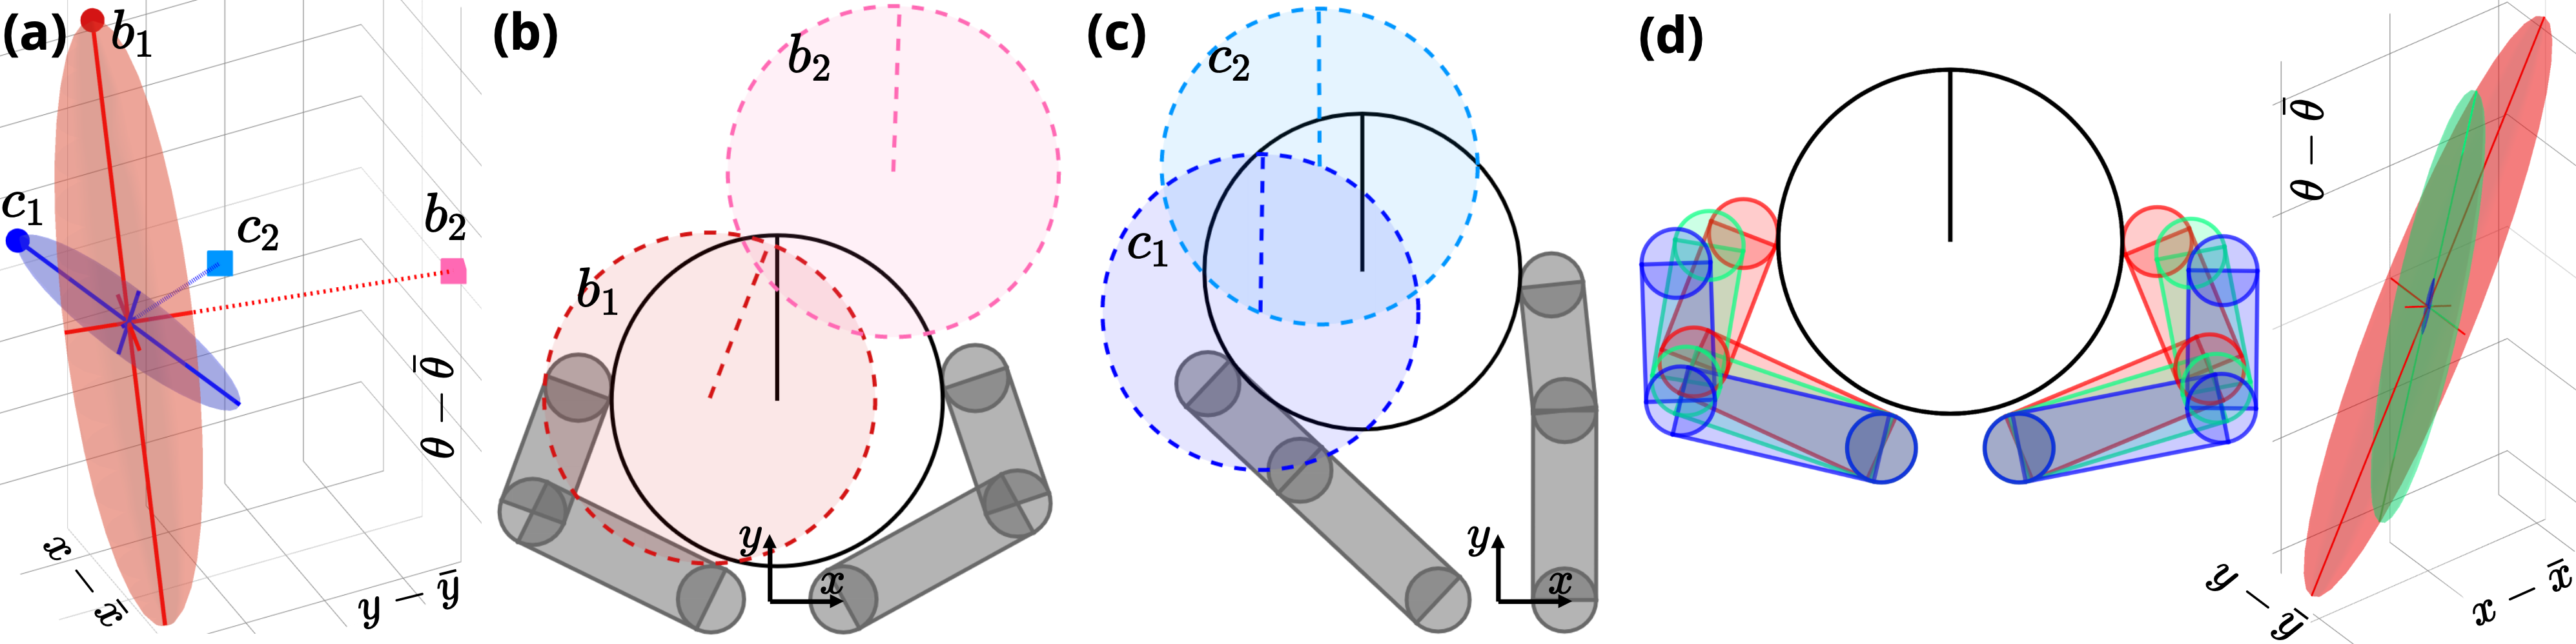
\includegraphics[width=1.0\textwidth]{figures/03_contact_rich_planning/reachability_planar_hand5.png}
\caption{(\textbf{a}) Two different sublevel sets $\mathcal{R}^\mathrm{u}_{\rho, \varepsilon, \gamma}$, represented as ellipsoids, shown in the space of $\qu$, with $\varepsilon = 1$, and $\gamma = 10^{-6}$. The ellipsoid centers are shifted to the origin for easy comparison. Red ellipsoid: $\mathcal{R}^\mathrm{u}_{\rho, \varepsilon, \gamma}$ for the system configuration in Fig. \ref{fig:reachability_planar_hand}b; blue ellipsoid: $\mathcal{R}^\mathrm{u}_{\rho, \varepsilon, \gamma}$ for the configuration in Fig. \ref{fig:reachability_planar_hand}c. Points $b_1$, $c_1$ are where ellipsoids' major axes intersect their boundaries. Points $b_2$, $c_2$ are points along the minor axes of the ellipsoids, and satisfy $\norm{b_1} = \norm{b_2}$ and $\norm{c_1} = \norm{c_2}$, where the norm is based on the standard Euclidean metric.
(\textbf{b}) The solid robots and objects represent the $\bar{q}$ at which the red $\mathcal{R}^\mathrm{u}_{\rho, \varepsilon, \gamma}$ in (a) is computed. The straight line on the puck indicates its orientation. The dashed dark red puck corresponds to the configuration $b_1$, and pink to $b_2$. Note that $b_1$ is easier to each than $b_2$.
(\textbf{c}) Similar to Fig. \ref{fig:reachability_planar_hand}b, the dashed dark blue puck correspond to $c_1$, and light blue to $c_2$. It is also easier to reach $c_1$ than $c_2$.
(\textbf{d}) The volume of $\mathcal{R}^\mathrm{u}_{\rho, \varepsilon, \gamma}$ shrinks as the fingers get further away from the puck. The ellipsoids on the right are color-coded to match the robot configurations on the left. Note that the blue ellipsoid is barely visible.}
\label{fig:reachability_planar_hand}

\end{figure*}

\subsection{The Local Mahalanobis Metric}

Consider the following problem: given the current configuration $\bar{q}$, and some queried configuration $q$, how can we formulate a distance metric $d(q;\bar{q})$ that is consistent with reachability characteristics of the system? We propose to utilize the locally linear model around the nominal configuration $\bar{q}$, that characterizes the local response of the next system configuration $q_+$ with respect to the movement of the actuated configurations $u$. This local model can be written as 
\begin{equation}
    q_+ = \mathbf{B}(\bar{q},\bar{q}^{\mathrm{a}})\underbrace{(u - \bar{q}^\mathrm{a})}_{\delta u} + c(\bar{q},\bar{q}^{\mathrm{a}})
\end{equation}
where the notation is consistent with the CQDC dynamics formulation in Sec.\ref{sec:convex_quasi_dynamic_contact_dynamics}; the input $u$ is the position command to the system), and $\mathbf{B},c$ are defined as \eqref{eq:linearization}. We note that the contribution of $\mathbf{A}$ term is zero since $\delta x = 0$.

Given such a local characterization, and a queried state $q$, we define the Mahalanobis metric as follows.
\begin{definition}
{\bf Local Mahalanobis Metric.}\normalfont \label{def:mahalanobis}
Given a nominal configuration $\bar{q}$, and queried configuration $q$, we define the Mahalanobis distance $d_\gamma$ of $q$ from $\bar{q}$ as follows:
\begin{equation}
\label{eq:metric}
\begin{aligned}
d_{\gamma}(q;\bar{q}) & \coloneqq \|q - \mu\|_{\mathbf{\Sigma}^{-1}_{\gamma}}=\textstyle\frac{1}{2}(q-\mu)^\intercal\mathbf{\Sigma}^{-1}_\gamma (q-\mu) \\
\mathbf{\Sigma}_{\gamma} & \coloneqq \mathbf{B}(\bar{q},\bar{q}^\mathrm{a})\mathbf{B}(\bar{q},\bar{q}^\mathrm{a})^\intercal + \gamma\mathbf{I}_n, \; \mu \coloneqq c(\bar{q},\bar{q}^\mathrm{a}).
\end{aligned}
\end{equation}
\end{definition}

The regularization $\gamma\mathbf{I}_n$ is added to ensure that $\mathbf{\Sigma}_{\gamma}$ is positive definite and the inverse $\mathbf{\Sigma}^{-1}_{\gamma}$ is well-defined. Note that the $\varepsilon$-sublevel set of this metric $d_\gamma(q;\bar{q})$, which we denote by $\mathcal{R}_{\varepsilon,\gamma}(\bar{q})$, describes an \emph{ellipsoid} that is centered at $\mu$ and has a shape matrix $\mathbf{\Sigma}^{-1}_\gamma$. We further motivate our construction of the metric by noting that this ellipsoid can be alternatively characterized (equivalent up to a regularization) by the following set, 
\begin{equation}
    \mathcal{R}_{\varepsilon}(\bar{q})\coloneqq \left\{\mathbf{B}(\bar{q},\bar{q}^{\mathrm{a}}) \delta u + c(\bar{q},\bar{q}^\mathrm{a})\; | \; \|\delta u\|\leq \varepsilon\right\}.
\end{equation}

This equivalence relation is exact when $\mathbf{B}$ has full row rank (i.e. the system is one-step controllable) and $\gamma=0$. On the other hand, if $\mathbf{B}$ loses rank, one of the principle axis of $\mathcal{R}_{\varepsilon}$ has a length of zero and the set becomes degenerate.

Finally, note that when $q-\mu \notin \mathbf{Range}(\mathbf{B})$, i.e. there is no actuation $u$ that can take the state $\bar{q}$ to the queried state $q$, the distance $ d_{\gamma}(q;\bar{q})$ is a large number dominated by the inverse of the regularization term $\gamma^{-1}$, which is consistent with the intuition that states that are harder to reach are further away.

\subsection{Metric on Smoothed Dynamics and Unactuated Objects}
\label{sec:smooth_metric}
As explained in the previous sections, the local model constructed using $\mathbf{B}$ may not be a very informative one for non-smooth systems with contact. In light of the various smoothing schemes introduced in Sec.\ref{sec:smoothdynamics} to alleviate this issue, we propose a metric by utilizing the linearization of the smooth surrogate $(\mathbf{B}_\rho,c_\rho)$, as opposed to those of the original contact dynamics, $(\mathbf{B},c)$. 

Furthermore, for systems where robots interact with unactuated objects through contact, we focus on the reachability of the objects, as the robots are actuated and can easily move to a desired configuration without contact. We combine smoothing and the object-centric reachability in the following variant of the Mahalanobis metric $d^\mathrm{u}_{\rho,\gamma}$, 
\begin{equation}
\label{eq:unactuated_mahalanobis_metric}
\begin{aligned}
d_{\rho,\gamma}^\mathrm{u}(q;\bar{q}) & \coloneqq \|q^\mathrm{u} - \mu^\mathrm{u}_\rho\|_{\mathbf{\Sigma}^{\mathrm{u}^{-1}}_{\rho,\gamma}}, \\
\mathbf{\Sigma}_{\rho,\gamma}^\mathrm{u} & \coloneqq \mathbf{B}^\mathrm{u}_\rho(\bar{q},\bar{q}^\mathrm{a})\mathbf{B}^\mathrm{u}_\rho(\bar{q},\bar{q}^\mathrm{a})^\intercal + \gamma\mathbf{I}_{n_\mathrm{u}},\\ 
\mu_\rho^\mathrm{u} & \coloneqq c_\rho^\mathrm{u}(\bar{q},\bar{q}^\mathrm{a}).
\end{aligned}
\end{equation}
where $\mathbf{B}^\mathrm{u}_\rho$ is formed by the rows of $\mathbf{B}_\rho$ corresponding to the unactuated DOFs, and $c_\rho^\mathrm{u}$ is defined similarly. Finally, we define $\mathcal{R}_{\rho,\varepsilon,\gamma}^\mathrm{u}(\bar{q})$ as the $\varepsilon$-sublevel set of $d^\mathrm{u}_{\rho,\gamma}(q;\bar{q})$. 

In the rest of this section, we give several examples that provide intuition into the local Mahalanobis metric $d^\mathrm{u}_{\rho,\gamma}$ and its sublevel set $\mathcal{R}^\mathrm{u}_{\rho,\varepsilon,\gamma}$. 

\begin{example} \normalfont \textbf{(Understanding $\B$ for Planar Systems)}
As shown in Sec. \ref{sec:quasi_static:artifacts}, \ref{sec:trajopt_setup:systems}), the CQDC dynamics \eqref{eq:q_dynamic_socp} simplifies to a QP \eqref{eq:q_dynamics_planar_qp} for planar systems. For reference, the QP \eqref{eq:q_dynamics_planar_qp} is reproduced below:
\begin{subequations}
\label{eq:q_dynamics_planar_qp_copy}
\begin{align}
\underset{\dq}{\minimize} \; &\frac{1}{2} \dq^\intercal \mathbf{Q} \dq + b^\intercal \dq, \; \text{subject to} \\
&(\Jn[i] + \mu_i \Jt[i]) \dq + \phi_i \geq 0, \; i \in \{1\dots\nC\}, \label{eq:q_dynamics_planar_qp_copy:constraint1}\\
&(\Jn[i] - \mu_i \Jt[i]) \dq + \phi_i \geq 0, \; i \in \{1\dots\nC\}. \label{eq:q_dynamics_planar_qp_copy:constraint2}
\end{align}
\end{subequations}
Recall that the contact Jacobian $\Jt[i]$ has only one row instead of two. We define $\J \in \R[(2\nC) \times n_q]$ by stacking the $\Jn[i] + \mu_i \Jt[i]$ and $\Jn[i] - \mu_i \Jt[i]$ from \eqref{eq:q_dynamics_planar_qp_copy:constraint1} and \eqref{eq:q_dynamics_planar_qp_copy:constraint2} into a single matrix, and partition $\J$ into $\Ju$ and $\Ja$ in a similar way as in \eqref{eq:contact_jacobian_i}.

More structure behind the $\mathbf{B}$ matrix (as defined in \eqref{eq:q_dynamics_AB}) can be revealed with a bit of linear algebra. We can work out by hand the application of the implicit function theorem to the KKT conditions of \eqref{eq:q_dynamics_planar_qp}, and the chain rule in \eqref{eq:DdqDu}, to obtain an explicit expression for $\B$:
\begin{subequations}
\label{eq:planar_B_structure}
\begin{align}
\mathbf{B} &=
\begin{bmatrix}
\Ba \\ 
\Bu
\end{bmatrix}
=
\begin{bmatrix}
\mathbf{I} - (h^2\Ka)^{-1} (\JaActive)^\intercal \mathbf{P} \JaActive \\
\Mu^{-1} (\JuActive)^\intercal \mathbf{P} \JaActive
\end{bmatrix}, \; \text{with}\\
\mathbf{P} &= \left[\JuActive \Mu^{-1} (\JuActive)^\intercal + \JaActive (h^2 \Ka)^{-1} (\JaActive)^{\intercal} \right]^{-1}.
\end{align}
\end{subequations}
where we assume $\JuActive$ and $\JaActive$ have full row rank. The tilde over a Jacobian indicates the sub-matrix formed by rows of the original matrix corresponding to the active constraints, i.e. contacts with non-zero contact forces.

%The robot actuation matrix, $\Ba$, is the difference between identity and a term that decreases as $\Ka$ grows, which is intuitively saying that a stiff robot usually goes to where it is asked to go. As for $\Bu$, it is noteworthy that the possible object motions in a specific contact mode live in the range of $(\JuActive)^\intercal$, the transpose of the active contact Jacobian. 

The structure in $\Bu$ explains why $\Bu_\rho$ is a good measure of the object's reachability when there is contact.
We can interpret $\mathbf{Range}(\JuActive^\intercal)$ as achievable object motions under the specific subset of active contacts.
By averaging $\Bu$ computed from different contacts which can be activated from the nominal $(\bar{q}, \bar{u})$, $\Bu_\rho$ summarizes possible object motions due to contact, in the form of $\mathbf{Range}(\JuActive^\intercal)$ weighted by $\Mu$ and $\mathbf{P}$. 

Furthermore, for a configuration with no active contacts, \eqref{eq:planar_B_structure} implies that $\Ba = \I$ and $\Bu = \mathbf{0}$, as both $\JaActive$ and $\JuActive$ are empty matrices in the absence of active contacts. This has the intuitive interpretation that under a $u$ that does not lead to contacts, the robot will move to where it is commanded to, and the object will remain still.

As $\mathbf{B}_\rho^\mathrm{u}$ is the expected value of $\mathbf{B}^\mathrm{u}$, it follows naturally from the above observation that the local distance metric $d_{\rho, \gamma}^\mathrm{u}$ tends to be dominated by the regularization $\gamma \mathbf{I}_{n_\mathrm{u}}$ for a nominal configuration $\bar{q}$ where robots and objects are far from making contact. In such cases, the probability that an action $u$ sampled from a distribution $\rho$ centered at $\bar{q}^\mathrm{a}$ leads to active contacts is low. As a result, in the Monte-Carlo estimation of $\mathbf{B}_\rho^\mathrm{u}$, such samples simply introduce $\mathbf{0}$ into the average, dragging the distance metric $d^\mathrm{u}_{\rho,\gamma}$ towards being dominated by the regularization.
\end{example}



\begin{example} \normalfont \textbf{(Metric on Planar Hand)}
\label{ex:planarhandreachableset}
We illustrate how the Mahalanobis metric can guide planning using the \code{PlanarHand} system first introduced in Sec. \ref{sec:trajopt_setup}.
As shown in Fig. \ref{fig:reachability_planar_hand}, the system lives in the $xy$ plane, with gravity pointing into the paper along the negative $z$ direction. The system consists of two actuated 2-link robotic fingers and an unactuated puck which is free to translate and rotate. Each finger can interact with the ball through frictional contacts along both links.

For a given $\qu$, the difficulty of reaching $\qu$ from $(\bar{q}, \bar{u})$ can be measured by the local Mahalanobis metric $d^\mathrm{u}_{\rho, \gamma}$, whose $1$-sublevel sets are shown in Fig. \ref{fig:reachability_planar_hand}a as ellipsoids. Although object configurations $b_1$ and $b_2$ are equidistant to the origin under the globally-uniform Euclidean metric, $b_1$ is considered much closer than $b_2$ under the local Mahalanobis metric (red ellipsoid). Indeed, in Fig. \ref{fig:reachability_planar_hand}b, reaching $b_1$ from the current puck configuration seems easier than reaching $b_2$. A similar observation can be made for the configuration in Fig. \ref{fig:reachability_planar_hand}c.

In addition, the local Mahalanobis metric also varies greatly from one configuration another, as evidenced by the difference between the blue and red ellipsoids in Fig. \ref{fig:reachability_planar_hand}a. This implies that a globally-uniform metric is rarely a good measure of reachability characteristics.

Lastly, the ellipsoid that corresponds to the $1$-sublevel set shrinks as the nominal state gets further away from the contact manifold, as shown in Fig. \ref{fig:reachability_planar_hand}d. This signifies that the configurations where the object is less accessible by the robot are naturally considered ``further away'' and can thus be avoided by the planner.
\end{example}


\section{RRT through Contact \label{sec:rrt_for_contact}}
\noindent We are now ready to present our smoothing-based enhancements to the vanilla RRT algorithm, which we reproduce in Alg. \ref{alg:rrt} to establish notations for our discussion. Our method enhances RRT by incorporating
(\textbf{i}) a reachability-aware $\Nearest$ operation based on the smoothed Mahalanobis metric on the unactuated objects $d_{\rho,\gamma}^\mathrm{u}$,
% a $\mathtt{Nearest}$ operation based on the object Mahalanobis reachability metric $d_{\rho,\gamma}^\mathrm{u}$ of individual nodes constructed on the smoothed dynamnics;
(\textbf{ii}) a fast $\Extend$ operation based on the projection of the subgoal to the range of $\mathbf{B}_\rho$; and
(\textbf{iii}) a contact sampling procedure which improves the reachability of nodes added to the tree.

We denote the RRT tree as $\mathcal{T}=(\mathcal{V},\mathcal{E})$ with vertex set $\mathcal{V}$ and edge set $\mathcal{E}$. Each node $q \in \mathcal{V}$ is simply a point in the configuration space of the system. 


\begin{algorithm}[t]
\caption{\textbf{RRT}}\label{alg:rrt}
\textbf{Input:} $q_{\mathrm{init}}, q_{\mathrm{goal}}, K$\;
\textbf{Output:} $\mathcal{T}$\;
$\mathcal{T} = \{q_{\mathrm{init}}\}$\;
\For {$k = 1, \dots, K$}{
    % \While{$\mathtt{IsInvalid}(v_{\mathrm{nearest}})$}
    $q_{\mathrm{subgoal}} = \mathtt{SampleSubgoal(p)}$\;
    $q_{\mathrm{nearest}} = \mathtt{Nearest}(q_{\mathrm{subgoal}})$\; \label{alg:rrt:nearest}
    % \EndWhile
    $q_{\mathrm{new}} = \mathtt{Extend}(q_{\mathrm{nearest}}, q_{\mathrm{subgoal}})$\;  \label{alg:rrt:extend}
    % \State $\mathcal{T}.\mathtt{Rewire(v_{\mathrm{new}})}$
    $\mathtt{AddNode}(q_{\mathrm{new}})$ \label{alg:rrt:add_node}\;
    \If{\texttt{GoalReached}}{$\textbf{break}$\;}
}
\end{algorithm}


\subsection{Nearest Node using Local Mahalanobis Metric}
As illustrated in Sec.\ref{sec:mahalanobis}, in particular by Example \ref{ex:planarhandreachableset}, a globally-uniform metric used by the vanilla RRT is usually a poor measure of reachability. Given a subgoal $q_{\mathrm{subgoal}}$, if the nearest node $q_{\mathrm{nearest}}$ is chosen under a globally-uniform metric, reaching $q_{\mathrm{subgoal}}$ from $q_{\mathrm{nearest}}$ may require large $u$ or even be dynamically infeasible. This will compromise RRT's ability to explore the configuration space, as trying to $\mathtt{Extend}$ towards a hard-to-reach $q_{\mathrm{subgoal}}$ typically returns a child node that is close to the parent node $q_{\mathrm{nearest}}$. In order to retain RRT's ability to efficiently explore under dynamics constraints, we use the smoothed Mahalanobis metric \eqref{eq:unactuated_mahalanobis_metric} instead of the usual Euclidean metric in the $\mathtt{Nearest}$ step:
\begin{equation}
q_{\mathrm{nearest}} = \text{argmin}_{q \in \mathcal{V}}\; d^{\mathrm{u}}_{\rho,\gamma}(q_{\mathrm{subgoal}}; q).
\end{equation}

\subsection{Dynamically Consistent Extension}
After choosing $q_{\mathrm{nearest}}$ from the tree $\mathcal{T}$, we need an action or a sequence of actions that moves the system from $q_{\mathrm{nearest}}$ to $q_{\mathrm{subgoal}}$ subject to the dynamics constraint. One feasible strategy to connect $q_{\mathrm{nearest}}$ to $q_{\mathrm{subgoal}}$ is to solve for an input sequence $\{u_t\}_{t=0}^{T-1}$ using a trajectory optimization algorithm such as Alg. \ref{alg:impc} \cite{karaman2010optimal}. However, the high computational cost of trajectory optimization motivates us to seek a simpler solution.

Fortunately, as a result of the farsightedness of quasi-static models, even an input sequence with $T = 1$ (i.e. a single time step) can steer the system fairly far away from $q_{\mathrm{nearest}}$. Although trajectory optimization with $T > 1$ can explore a larger region around $q_{\mathrm{nearest}}$, we find in practice that a single time step is sufficient for $\Extend$ to effectively grow the RRT tree $\mathcal{T}$.

We present the modified $\Extend$ that uses a single time step in Alg. \ref{alg:extend}. The input $u$ is computed by projecting $(q^\mathrm{u}_{\mathrm{subgoal}} - \mu_\rho^\mathrm{u})$ to $\mathbf{Range}(\Bu_\rho)$ using least squares (Line \ref{alg:extend:lstsq}), which is significantly cheaper than solving trajectory optimization. Afterwards, we normalize the input and multiply it by some stepsize $\varepsilon$. The scaled input is then passed to the forward dynamics to obtain a new node. Crucially, we use the actual dynamics $f$ as opposed to the smooth surrogate dynamics $f_\rho$ (Line \ref{alg:extend:rollout}). This ensures that while the search for the next action relies on the smoothed model, the actual path is dynamically consistent under the original non-smooth contact dynamics (i.e. CQDC). 

\begin{algorithm}
\caption{$\mathtt{Extend}$}\label{alg:extend}
\textbf{Input:} $q_{\mathrm{nearest}}, q_{\mathrm{subgoal}}$\;  \textbf{Output:} $q_{\mathrm{new}}$\;
$\delta u^\star = \mathrm{argmin}_{\delta u} \|\Bu_\rho \delta u + c_\rho^\mathrm{u} - q_{\mathrm{subgoal}}^\mathrm{u} \|$ \label{alg:extend:lstsq} \;
% $\varepsilon = \min(\varepsilon_\mathrm{max}, \norm{\delta u^\star})$ \label{alg:extend:cap}\;
\algorithmicreturn  $\; f(q_{\mathrm{nearest}}, q_{\mathrm{nearest}}^\mathrm{a} + \varepsilon \cdot \delta u^\star / \|\delta u^\star\|)$ \label{alg:extend:rollout}\;
\end{algorithm}


\subsection{Contact Sampling}\label{sec:contactsampling}
A node $q$ where robots and objects are far from making contacts hinders the growth of the RRT tree for two reasons. First, such nodes are considered far away under the local Mahalanobis metric from most sampled $q_\mathrm{subgoal}$, as the sublevel sets of their Mahalanobis distance metric have small volume (e.g. Fig. \ref{fig:reachability_planar_hand}d). As a result, adding such nodes to the tree simply increases ``deadweight'' without improving coverage of the state space. Moreover, when such a node is chosen by $\Nearest$, the $\Extend$ operation that follows often results in another non-contact configuration.

To reduce the number of such nodes in $\mathcal{T}$ and improve exploration during tree growth, the $\Extend$ operation is replaced, with some probability, by a new operation called $\ContactSample$. $\ContactSample$ takes $q_\mathrm{nearest}$ as input, and creates another node with a better local metric by fixing $q_\mathrm{nearest}^\mathrm{u}$ and finding an informative $q_\mathrm{nearest}^\mathrm{a}$ that makes contact with the object. 

The $\ContactSample$ operation is essential for adequate exploration of the robot's state space, and needs to be designed differently for different robots. 
As an example, we briefly describe how $\ContactSample$ is implemented for the three robots shown in Fig. \ref{fig:rrt_tasks}, which are used in our experiments in Sec. \ref{sec:rrt_results}. 
\begin{itemize}
\item \code{PlanarPushing}. The robot (the red sphere) is placed at a random point sampled on the perimeter of the box. 
\item \code{PlanarHand}. The robot consists of two fingers that can be treated as two-link robot arms. There are two different ways for the robot to contact the sphere: 
(\textbf{i}) \emph{enveloping} grasps, where for each finger, we start with the finger straight and horizontal, and then rotate each joint towards the ball until all links are touching the ball; 
(\textbf{ii}) \emph{pinch} grasps, where for each finger, we sample a point on the sphere, and solve inverse kinematics to find a finger configuration that touches the ball at the fingertip. 
\item \code{AllegroHand} (in all 4 systems with the hand). We start with the hand open and near the object (for \code{AllegroDoor} the object is the door knob). We then close the hand along a randomly picked direction in the robot's joint space until the object is ``grasped''.  The direction is generated by a weighted average of several EigenGrasps directions \cite{eigengrasp}, where the weights are sampled randomly. 
\end{itemize}  

Contact sampling introduces non-physical behavior where the robot teleports from one configuration to another. This is not a problem when the object can sustain static equilibrium without the actuated DOFs that need to teleport. For instance, in \code{AllegroHand}, when the ball is supported by the palm, the fingers are free to move around the ball to regrasp. In contrast, if \code{AllegroHand} were facing downwards, the ball would fall under gravity if it were not secured by some of the fingers. Although this is a limitation of our current contact sampling implementation, we believe this can be resolved by a more sophisticated contact sampler which moves some of the actuated DOFs while keeping the object in static equilibrium with the rest. 

\subsection{Effectiveness of Proposed Enhancements \label{sec:rrt_contact_effectiveness}}

\begin{figure*}
\centering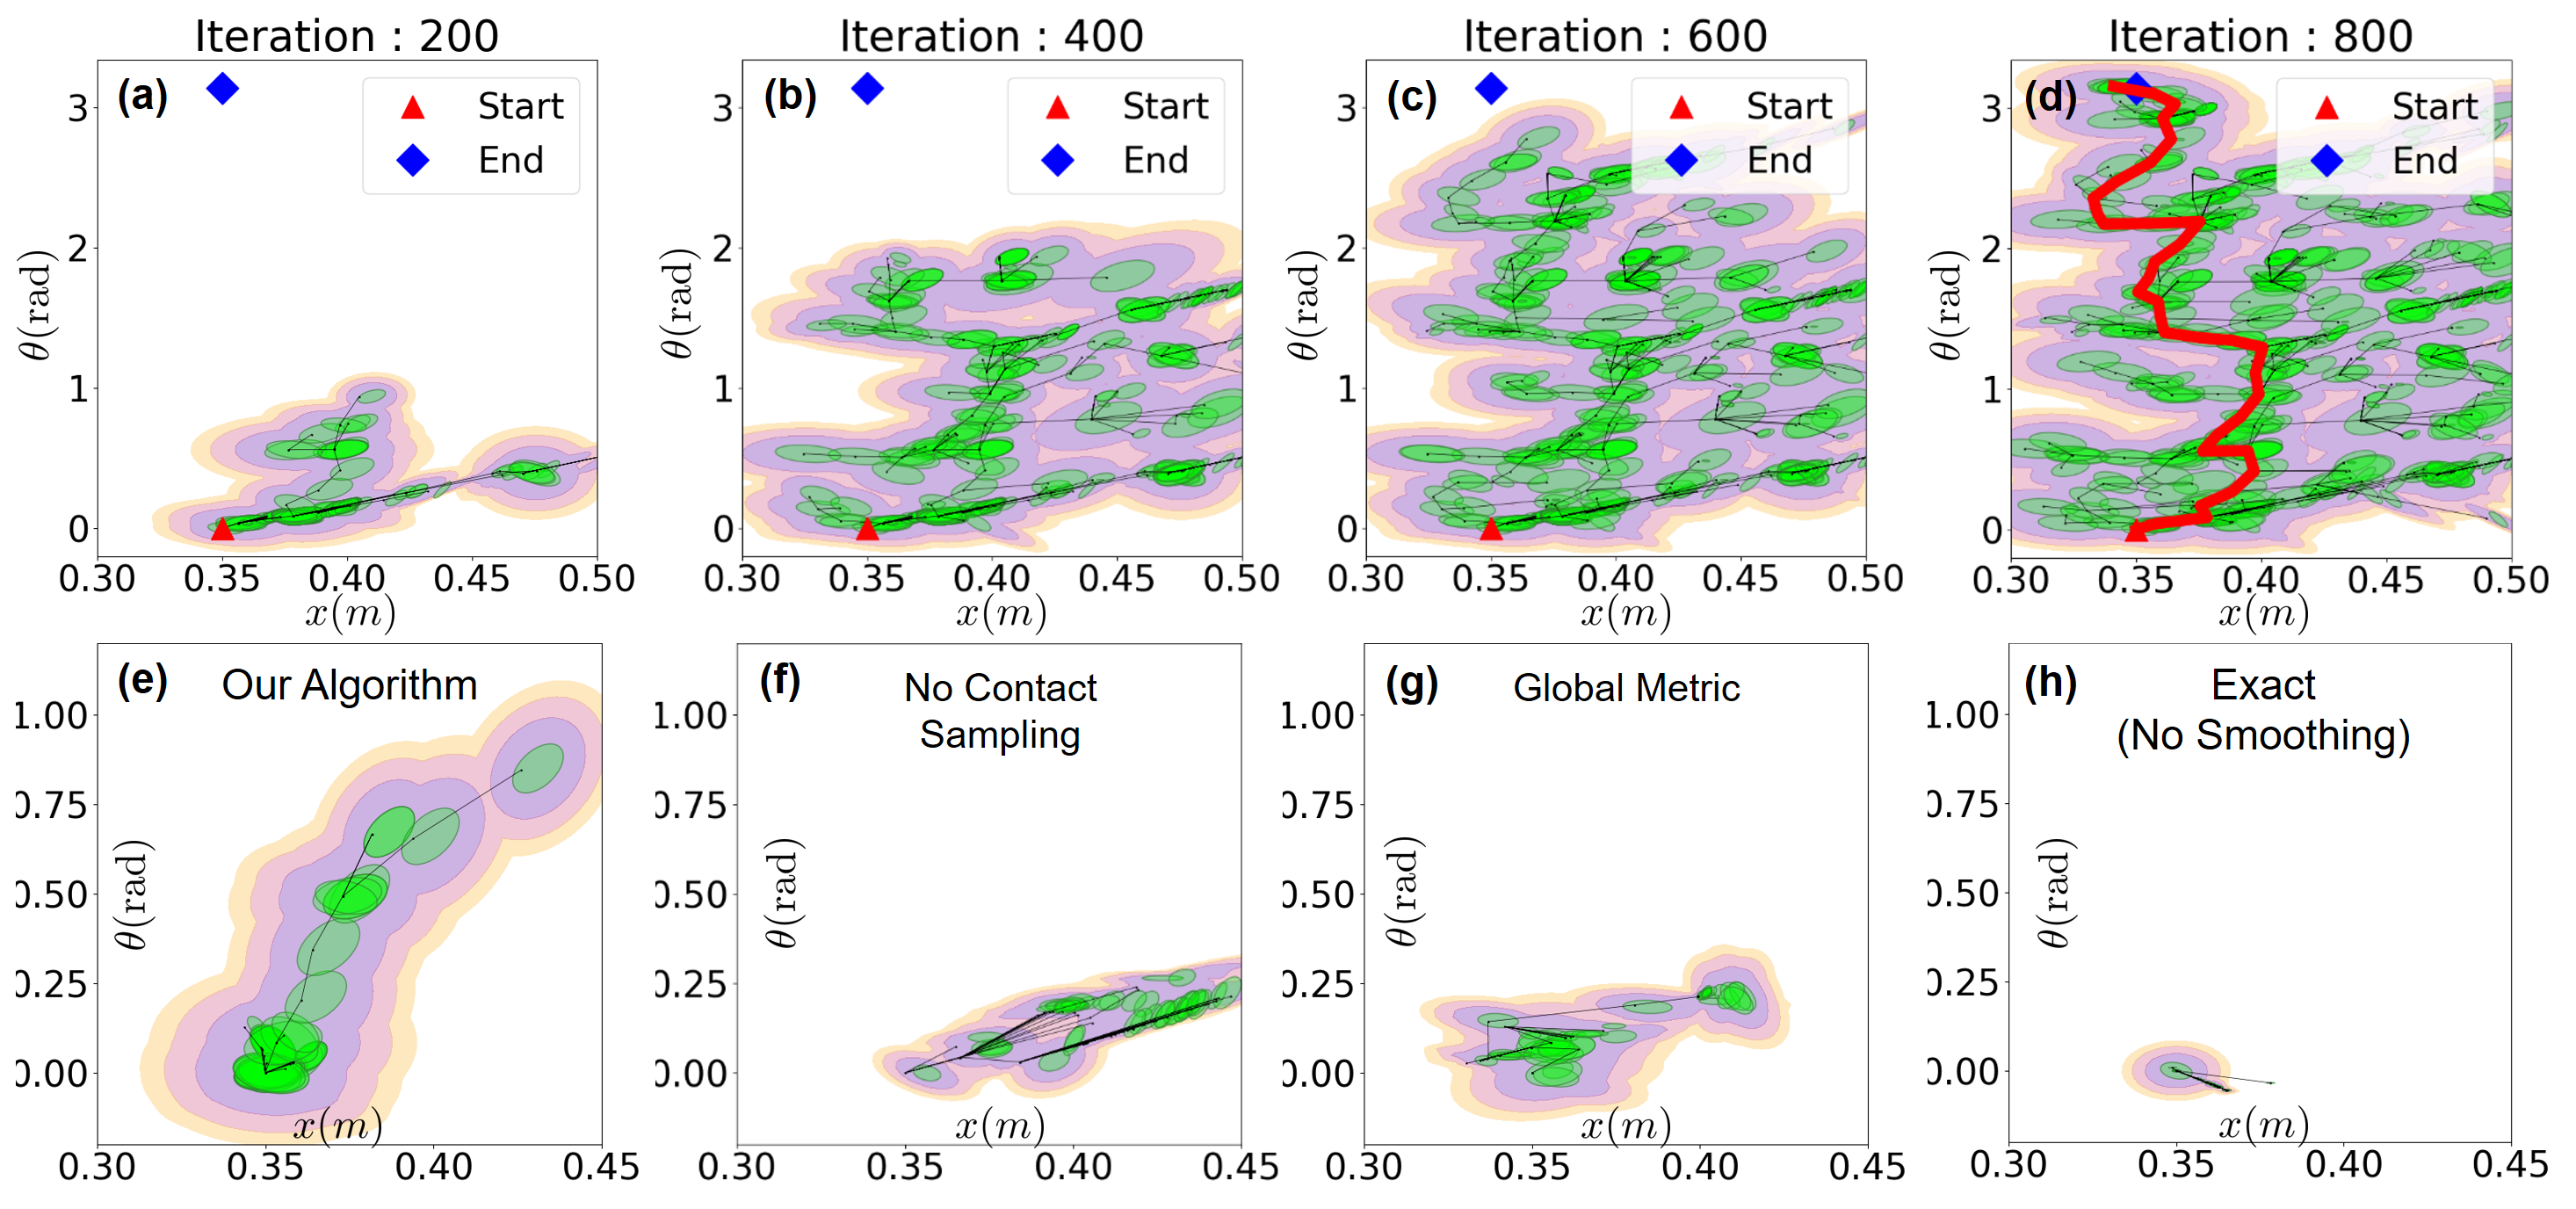
\includegraphics[width = 1.0\textwidth]{figures/03_contact_rich_planning/iteration_plot_combined_horizontal.png}
\caption{\textbf{(a-d)} RRT trees, shown in the space of $\qu$, at different iterations of a complete run of the enhanced RRT for the \code{PlanarHandFixedY} system. The contours are the sub-level sets of the local Mahalanobis metric of the nodes. The path from start ($q_\mathrm{init}$) to goal ($q_\mathrm{goal}$) is highlighted in red in the final tree of \textbf{(d)}. \textbf{(e-h)} Visualization of RRT trees with the same number of nodes (50) but grown with different methods. (\textbf{e}) Tree grown with our algorithm; (\textbf{f}) without contact sampling; (\textbf{g}) using a globally uniform weighted Euclidean metric; (\textbf{h}) using exact gradients without smoothing. Note that our method achieves the best coverage of the space of $\qu$.}
\label{fig:degenerate}
\end{figure*}

We introduce a new system with a 2-dimensional object configuration space to illustrate the effectiveness of the proposed RRT enhancements:
\begin{itemize}
\item {\bf Planar Hand with fixed $y$, (2,4,13)}. A simplified version of the \code{PlanarHand} system in Sec. \ref{sec:trajopt_setup}. We fix the $y$-coordinate of the object, so that $\qu = (x, \theta)\in \R[2]$ can be easily plotted on paper. 
\end{itemize}

As shown in Fig. \ref{fig:degenerate}e, the vanilla RRT enhanced with the proposed $\Nearest$, $\Extend$ and $\ContactSample$ achieves good coverage of the space of $\qu$, which is crucial for RRT to adequately explore the configuration space and find a path to $q_\mathrm{goal}$. In contrast, tree growth is stuck around the root without contact sampling (Fig. \ref{fig:degenerate}f) or the local metric (Fig. \ref{fig:degenerate}g).

We also illustrate how the tree grows throughout a complete run of the enhanced RRT in Fig. \ref{fig:degenerate}a-d. Even with the proposed enhancements, tree growth can get stuck at times. This is characterized by a specific type of subgraph of the tree which we call a ``broom''. A broom consists of one parent node with many child nodes, and is formed by repeated unsuccessful attempts to grow towards different subgoals from the same parent node. The occasional appearance of brooms is a sign that the proposed enhancements are not perfect. Nevertheless, the enhanced RRT is able to quickly branch out into empty part of the configuration space, and sufficiently cover the space as the tree grows. 

\subsection{Final Path Refinement}

The final path returned by the RRT algorithm is visually plausible, yet suffers from two minor drawbacks: (\textbf{i}) RRT tends to produce randomized paths that can be shortened, and (\textbf{ii}) the big step size used in the $\Extend$ operation creates some non-physical artifacts due to Anitescu’s convex relaxation of the Coulomb friction model (Sec.\ref{sec:convex_quasi_dynamic_contact_dynamics}). 

To mitigate these issues, we refine the RRT plan using trajectory optimization \cite{lgp,terry} and short-cutting \cite{shortcutting}. 
We first divide the RRT path into segments punctuated by $\ContactSample$ operations. We call these segments contact-rich as they involve contact-based interactions between the object and the robot. 
We shortcut the sequence of trajectories by (\textbf{i}) removing consecutive $\ContactSample$ steps, and (\textbf{ii}) truncating each segment if there is no movement in $\qu$. 
Then, for each contact-rich segment, we run trajectory optimization (Alg.\ref{alg:impc}) with a smaller time step $h$, using the RRT path segment as the initial guess. This not only smooths the final path, but also ensures that each trajectory segment is more physically realistic.
Finally, we connect adjacent contact-rich segments with a collision-free robot trajectory created by a collision-free RRT. We assume that the object configuration remains unchanged during the collision-free segment.

We find that combining these two strategies is effective in creating shorter and more physically realistic trajectories. 

\begin{figure*}
\centering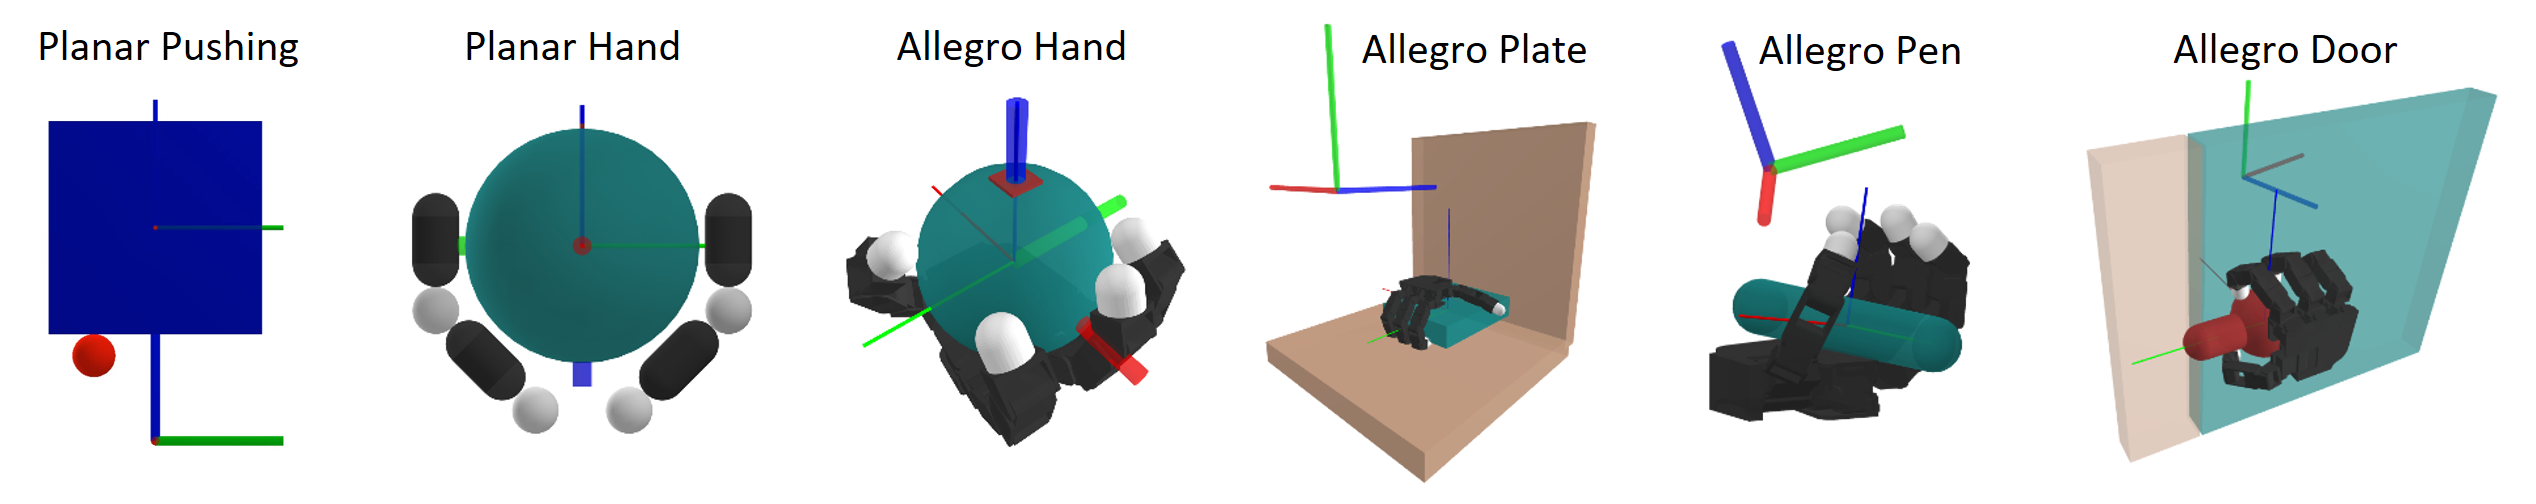
\includegraphics[width = 1.0\linewidth]{figures/03_contact_rich_planning/rrt_systems_pagewide.png}
\caption{Tasks for RRT. Similar to Fig. \ref{fig:trajoptvis}, the thicker frame denotes the goal, and the thinner frame the initial configuration of the object.}
\label{fig:rrt_tasks}
\end{figure*}



\section{Results \& Discussion \label{sec:rrt_results}}
\noindent In this section, we apply our algorithm on difficult 3D contact-rich manipulation problems previously only tackled by heavy offline approaches in RL \cite{rajeswaran2018learning, chen2022system}, and illustrate that we can generate plans on the order of a minute of online compute time, all on the CPU, which shows the efficacy of our method.
The experiments in this section are designed to validate the following four hypotheses.
\begin{enumerate}
\item Using the smooth surrogate greatly improves the performance over using the exact dynamics for linearization.
\item The equivalence of smoothing schemes establishes that analytic and randomized smoothing will have similar levels of performance empirically, with analytic smoothing showing superior computation time.
\item Using the Mahalanobis distance metric improves performance over a globally uniform distance metric.
\item Contact sampling greatly aids sample efficiency of the algorithm.
\end{enumerate}

\subsection{Experiment Setup \label{sec:rrt_experiment_setup}} 
To test the efficacy of our algorithm and the above stated hypotheses, we run our algorithm to reach more challenging goals than the trajectory optimization examples in Sec. \ref{sec:trajopt_setup:systems}, as well as on 3 more contact-rich tasks on 3 new systems defined below.
\begin{enumerate}
    \item {\bf Pen Placement (6,19,24)}. The robot hand needs to both translate and rotate the pen \cite{rajeswaran2018learning} to the desired configuration.
    \item {\bf Plate Pickup (6,19,42)}. The robot has to exploit the external contact between the plate and the wall \cite{cheng2021contact}, showing extrinsic dexterity \cite{extrinsic}.
    \item {\bf Door Opening (2,19,22)} \cite{rajeswaran2018learning} involves reasoning about a constrained system, where the handle must be rotated first before the door can be pushed open.
\end{enumerate}
The definition of the number tuples is identical to Sec.\ref{sec:trajopt_setup:systems}.

The contact-rich planning tasks are illustrated in Fig. \ref{fig:rrt_tasks}.
We design the tasks so that solving any of them with a single run of trajectory optimization is expected to fail due to their difficulty and the resulting non-convexity of the problem. 


To compare our algorithm with different baselines, we rate the quality of planners using two metrics:
\begin{enumerate}
    \item {\bf Iteration vs. Minimum distance to goal}.  we measure the distance between the goal and the tree, defined by $\min_{q\in\mathcal{V}} \|q^\mathrm{u} - q_\textrm{goal}^\mathrm{u}\|$ for every iteration. A successful planning algorithm would eventually reach the vicinity of the goal asymptotically, driving this metric to zero. 
    \item {\bf Iteration vs. Packing Ratio}. To characterize the \emph{exploration} performance of RRT, we do a Monte-Carlo estimation of the \emph{packing ratio}, which is defined as the volume of the space occupied by the reachability ellipses, divided by the total volume of some workspace limit for the unactuated objects. The workspace limit is the set from which subgoals are sampled when running RRT. More formally, we define the numerator as
    \begin{equation}
        V_{\mathrm{reachable}} = \textbf{vol}\big(\{q^\mathrm{u} | \min_{\bar{q}\in\mathcal{V}} d^\mathrm{u}_{\rho,\gamma}(q; \bar{q}) \leq \eta\}\big)
    \end{equation}
    where $\eta$ is some threshold on the distance metric. The Monte-Carlo estimate of $V_{\mathrm{reachable}}/V_{\mathrm{workspace}}$ can be computed by drawing $N$ samples within the workspace and counting how many of them belong to $V_{\mathrm{reachable}}$. A good planner should asymptotically reach a ratio of $1$ if the system can reach all points in the workspace.
\end{enumerate}

\begin{figure}
\centering
\subfloat[Planar Pushing.]{
	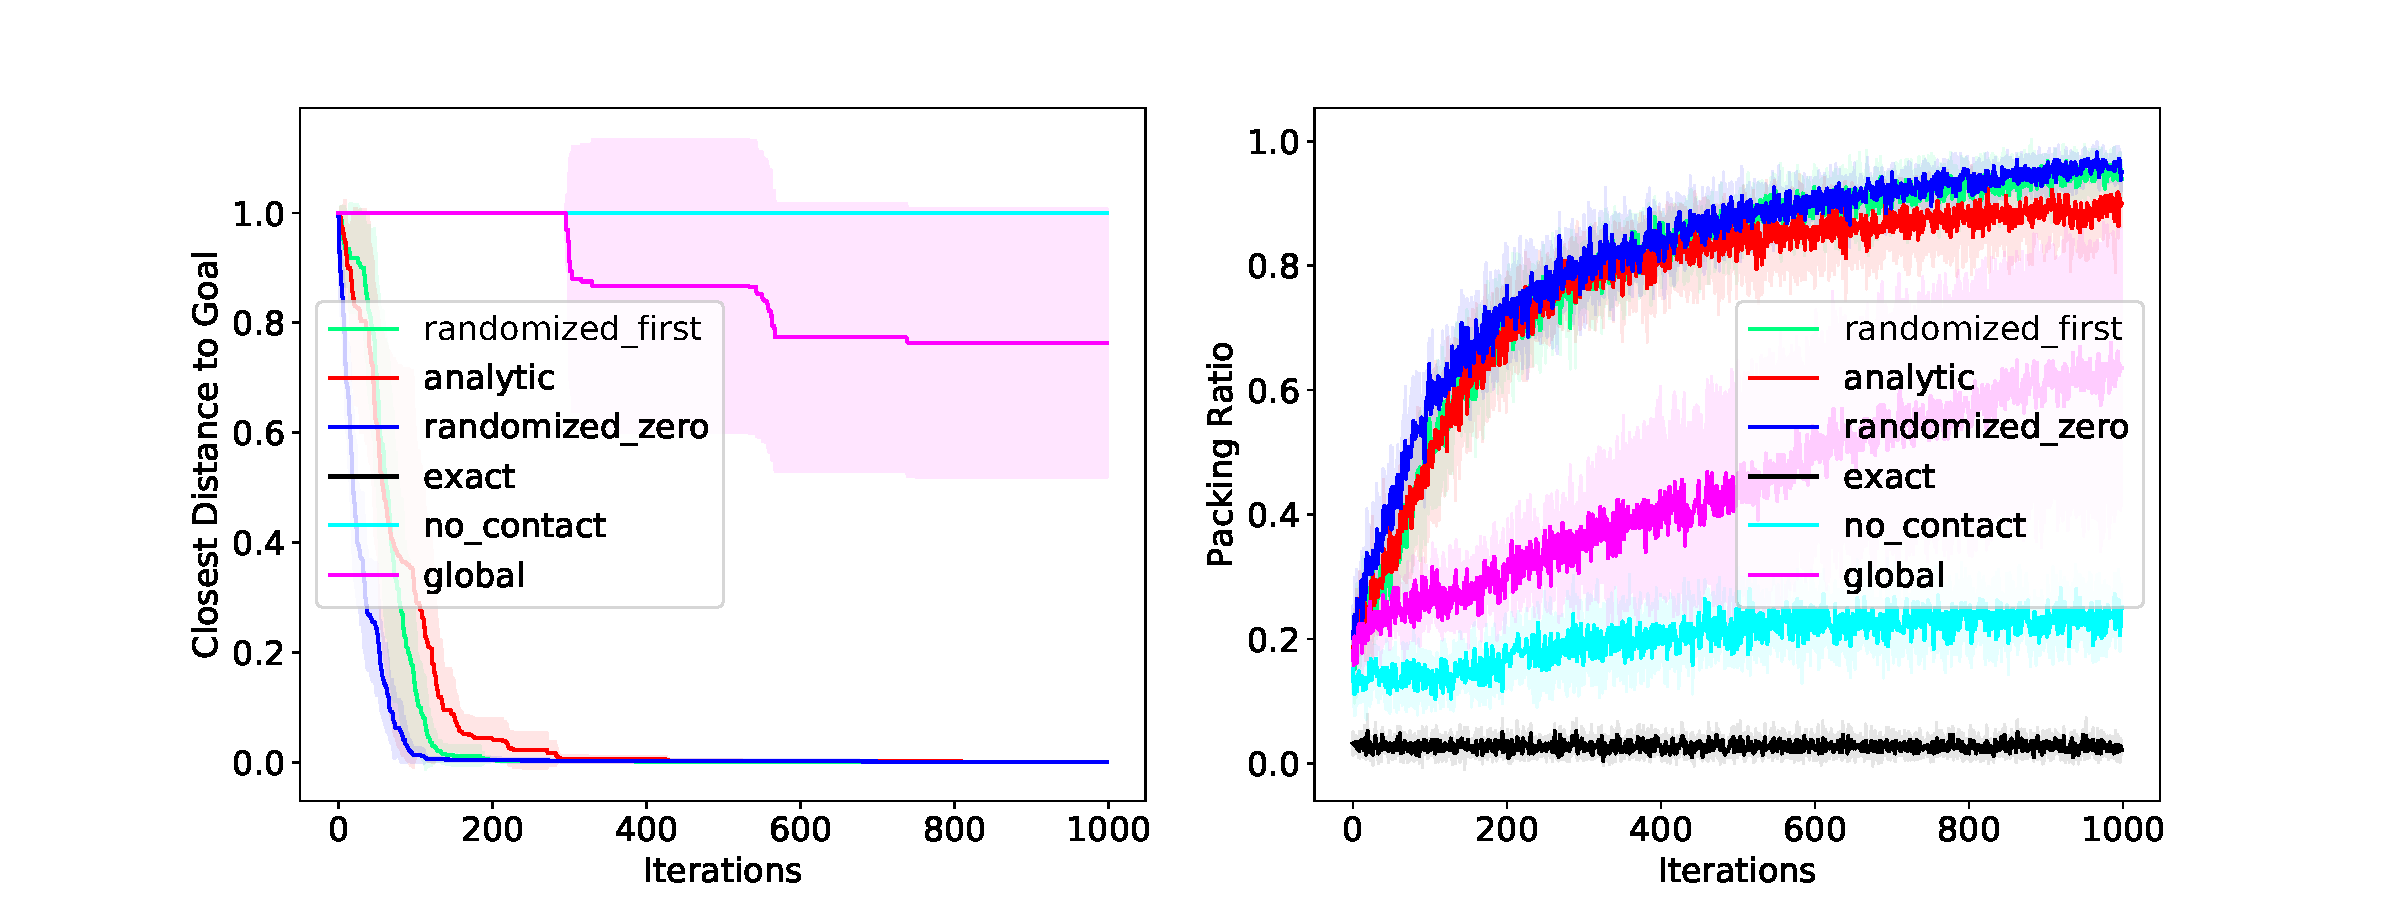
\includegraphics[width=0.485\linewidth]{figures/03_contact_rich_planning/rrt_results/planar_pushing_renamed.pdf}
}
\subfloat[Allegro Plate.]{
	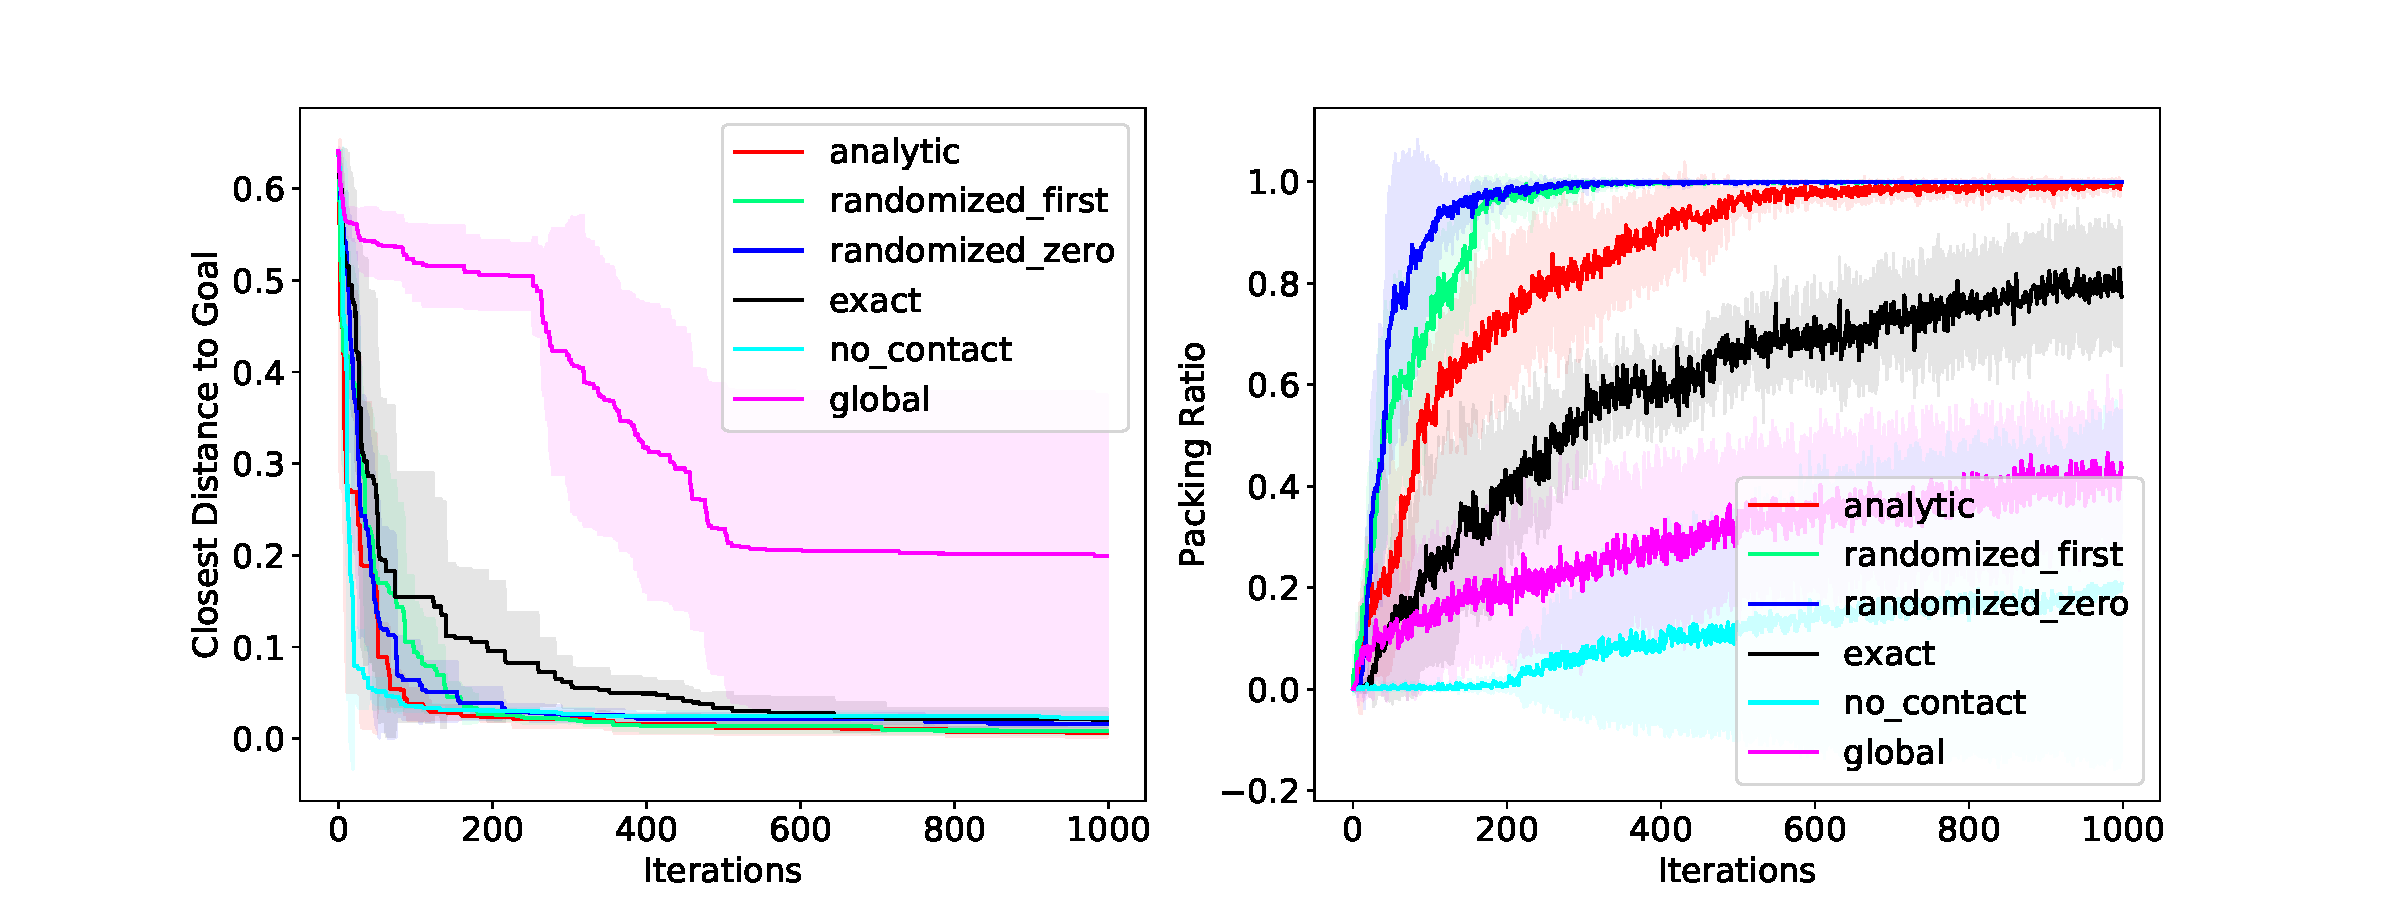
\includegraphics[width=0.485\linewidth]{figures/03_contact_rich_planning/rrt_results/allegrohandplate.pdf}
} \\
\vspace{-0.2cm}
\subfloat[Planar Hand.]{
	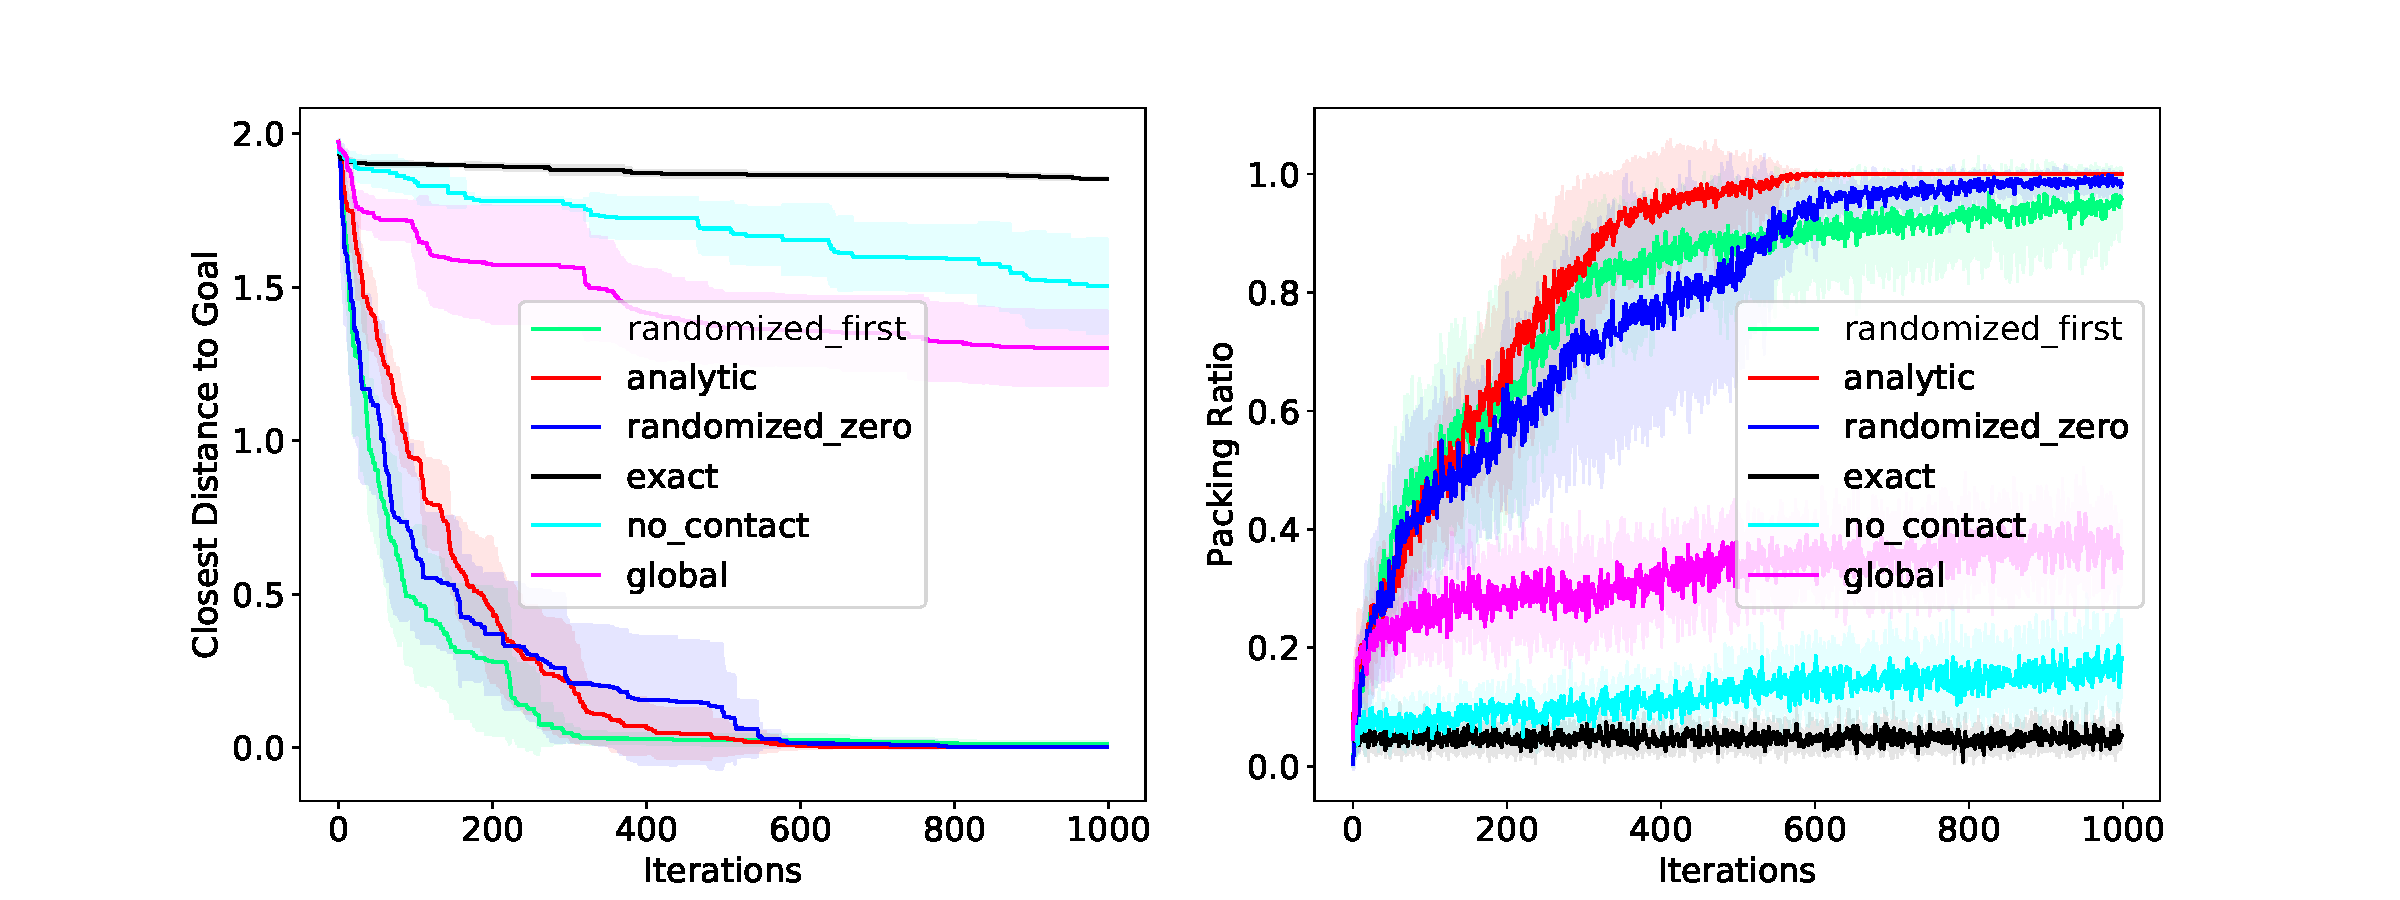
\includegraphics[width=0.485\linewidth]{figures/03_contact_rich_planning/rrt_results/planar_hand_renamed.pdf}
}
\subfloat[Allegro Pen.]{
	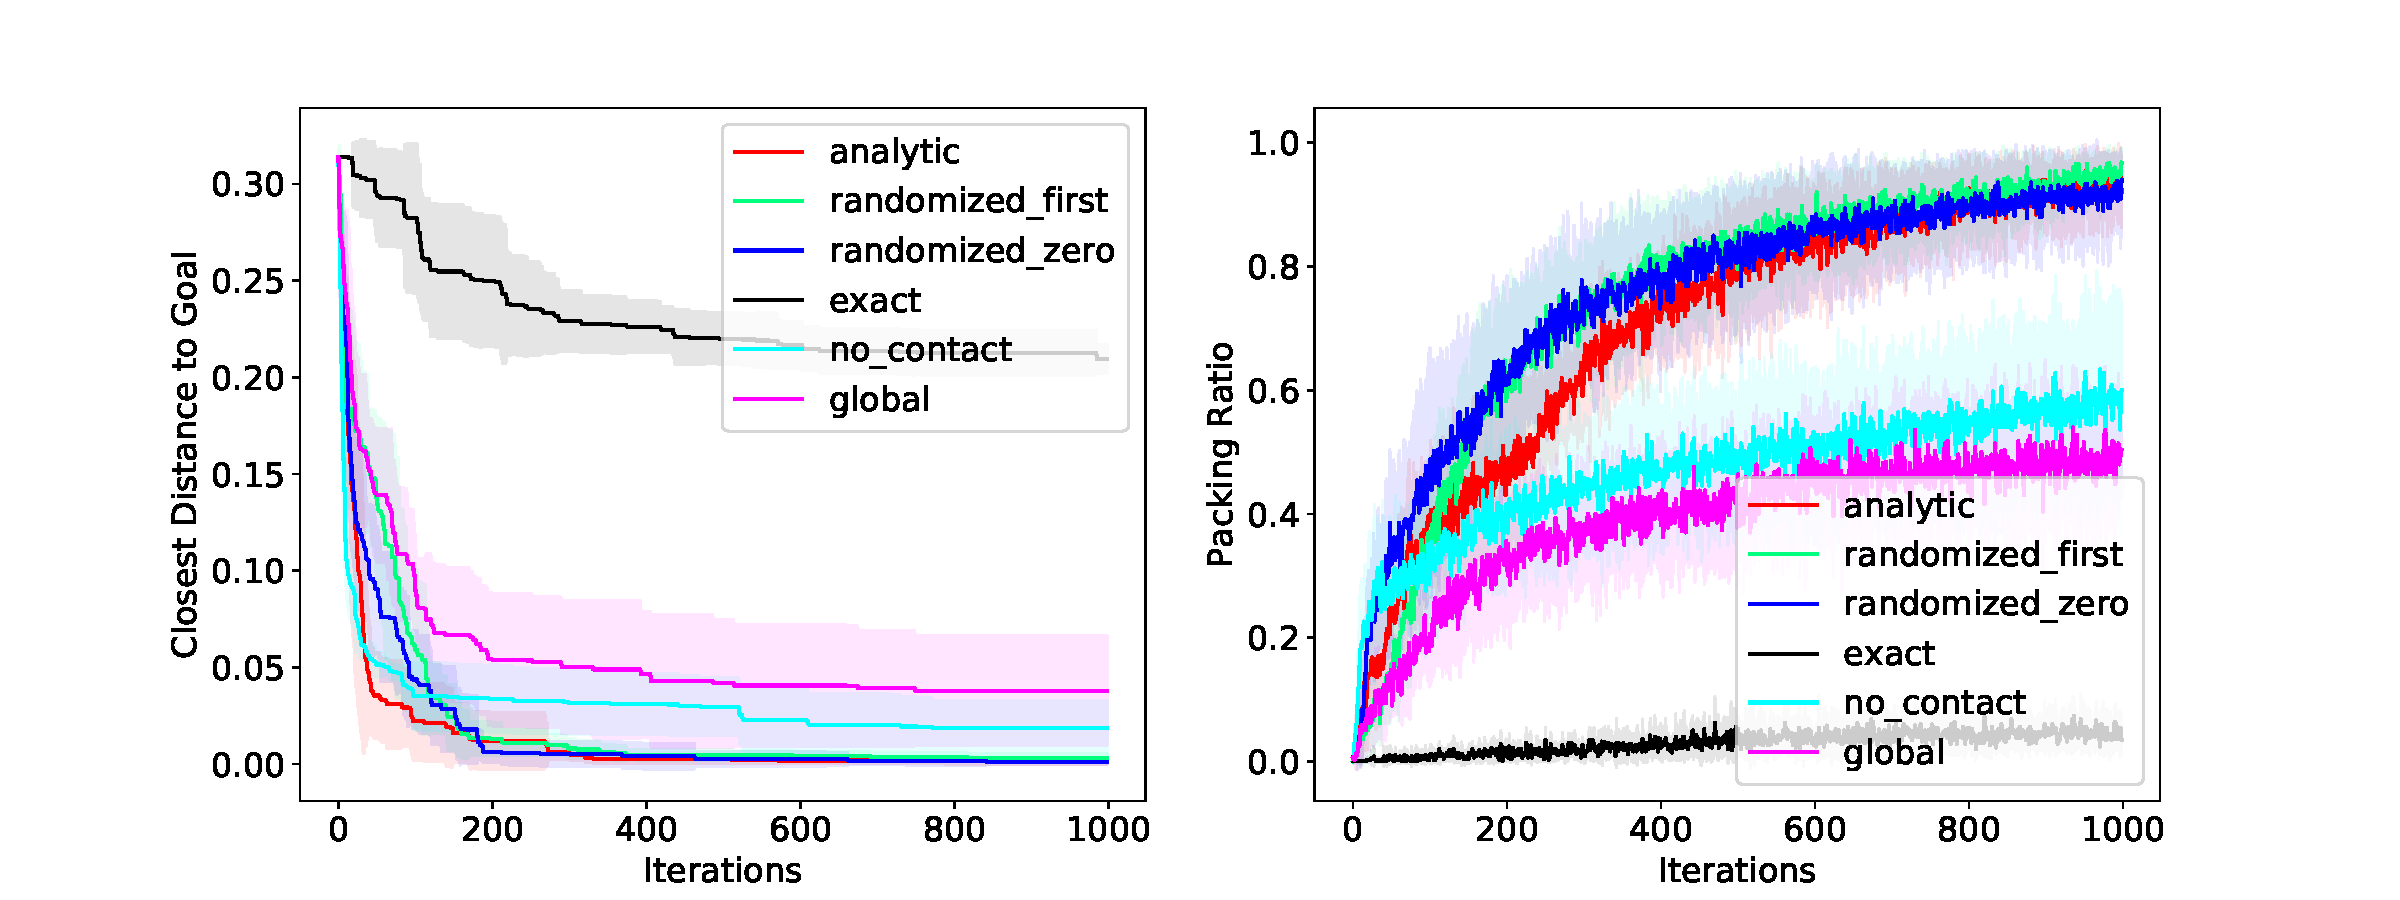
\includegraphics[width=0.485\linewidth]{figures/03_contact_rich_planning/rrt_results/allegrohandpen.pdf}
} \\
\vspace{-0.2cm}
\subfloat[Allegro Hand.]{
	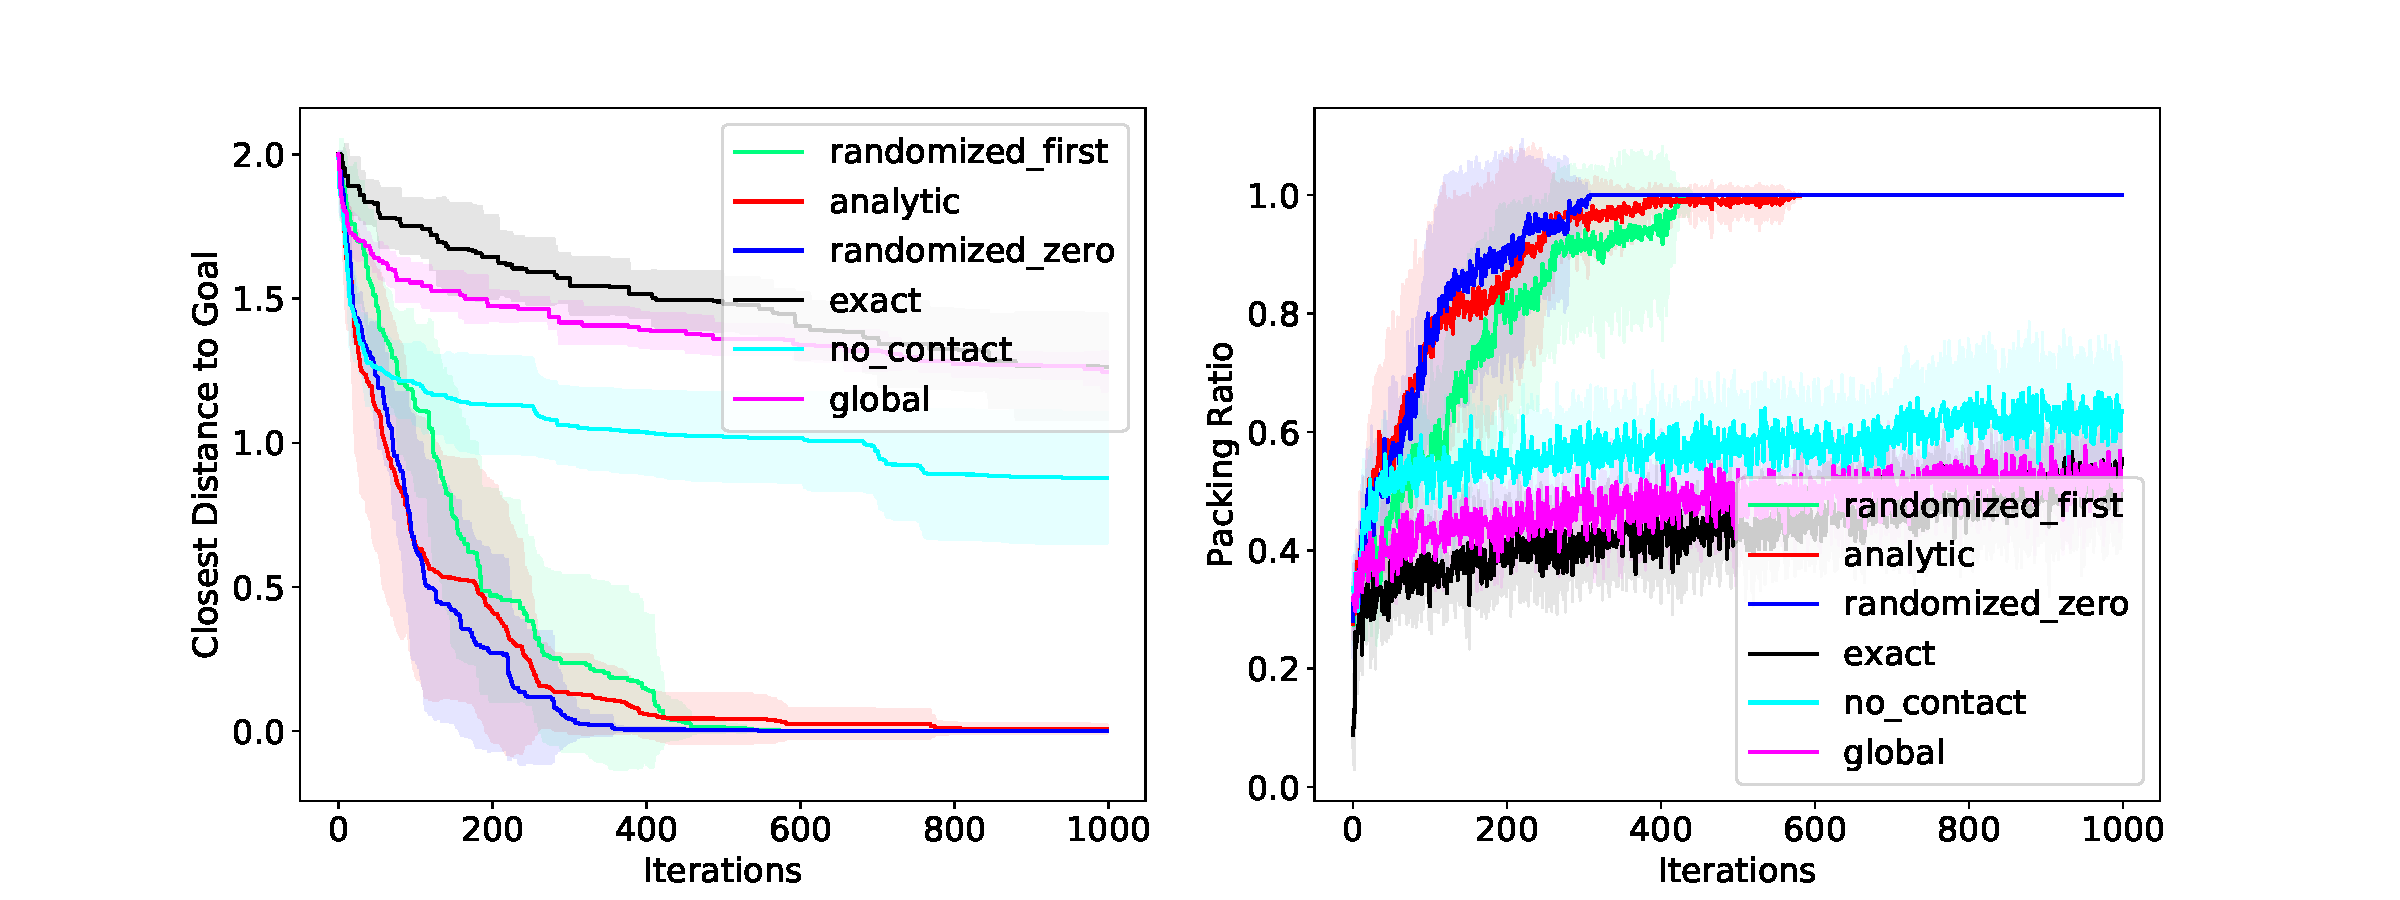
\includegraphics[width=0.485\linewidth]{figures/03_contact_rich_planning/rrt_results/allegrohand.pdf}
}
\subfloat[Allegro Door.]{
	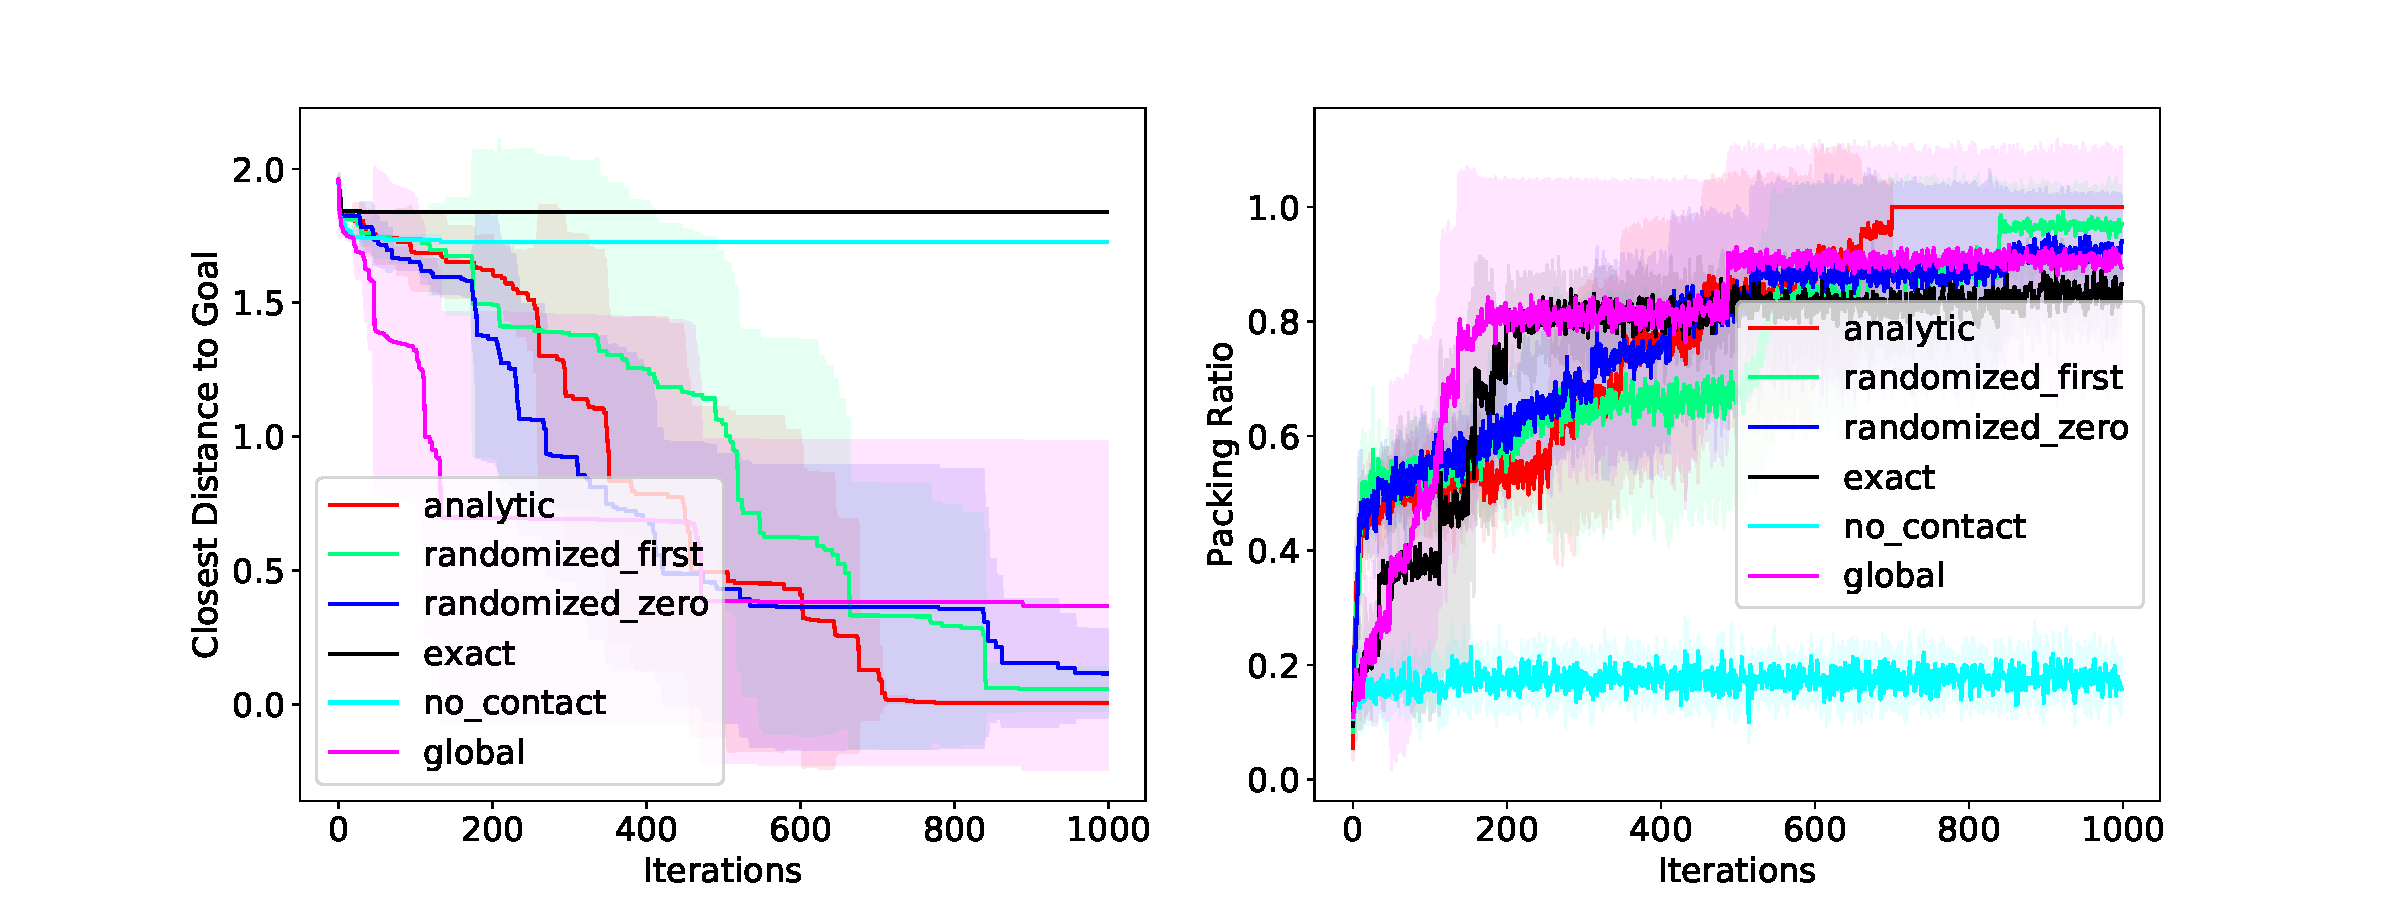
\includegraphics[width=0.485\linewidth]{figures/03_contact_rich_planning/rrt_results/allegrohanddoor.pdf}
}
\caption{Planning performance for the tasks in Fig. \ref{fig:rrt_tasks}. Results include running RRT with the enhancements proposed in Sec. \ref{sec:rrt_for_contact} using the three smoothing schemes from Sec. \ref{sec:smoothdynamics}, as well as the three ablation studies proposed in Sec. \ref{sec:rrt_experiment_setup}.}
\label{fig:rrtperformance}
\end{figure}

\iffalse
\begin{table*}[thpb] \label{tab:trajoptresults}
\centering
\begin{tabular}{|| c | r | r | r | r | r | r || r | r | r | r | r | r || } 
 \hline
 Problem & \multicolumn{2}{||c||}{PlanarPushing} & \multicolumn{2}{||c||}{PlanarHand} & \multicolumn{2}{||c||}{AllegroHand} &
 \multicolumn{2}{||c||}{AllegroPlate} & 
 \multicolumn{2}{||c||}{AllegroPen} & 
 \multicolumn{2}{||c||}{AllegroDoor} 
 \\\hline
 Method & Cost & Time(s) & Cost & Time(s) & Cost & Time(s) & Cost & Time(s) & Cost & Time(s) & Cost & Time(s)  \\ \hline\hline

    Analytic && 3.25  && 10.32 && 31.01 && 117.16 && 24.84 && 12.42  \\
    Randomized  && 7.50 && 21.34 && 80.12 && 161.64 && 86.12 && 34.55\\
    RandomizedZero && 7.40 && 21.00 && 82.00 && 168.11 && 81.23 && 33.80 \\
    Exact && - && - && - && - && - && - \\
    NoContact && - && - && - && - && - && - \\
    Global && - && - && - && - && - && - \\\hline
\end{tabular}
\caption{Minimum cost and running time achieved by different methods. Number of iterations run. Every run except \code{AllegroDoor} was run for $1000$ iterations. We choose to not display running time for the ablation options since they are slight variations of Analytic with comparable running times.}
\label{table:rrtrresults}
\end{table*}
\fi 

For both metrics, the performance of our RRT algorithms averaged over 5 runs is plotted in Fig. \ref{fig:rrtperformance} for different smoothing schemes, as well as ablations of different choices we made for the algorithm. In particular, we run three variations of our algorithm that misses a crucial ingredient.
\begin{enumerate}
    \item \textbf{Exact}. We replace the linearization of the smooth surrogate $\mathbf{B}_\rho$ with the exact linearization $\mathbf{B}$, used for both extension and metric computation.
    \item \textbf{NoContact}. We do not allow contact sampling (Sec.\ref{sec:contactsampling}) in this variant of the algorithm.
    \item \textbf{Global}. Instead of the local Mahalanobis metric, we use a globally uniform metric during the $\Nearest$ step of the algorithm. For our experiments, we use a carefully-chosen weighted Euclidean norm. 
\end{enumerate}
% By showing the results, we aim to show that the choices we made in the design of the algorithm were necessary.


\subsection{Results \& Discussion}

We plot the results of our experiments in Fig. \ref{fig:rrtperformance}, and display the running time of our algorithm using the three different smoothing schemes in Table \ref{table:rrtrresults}. We discuss some of our findings from the experiment, in the context of our hypotheses in the beginning of this section.

\begin{table}[thpb]
\centering
\begin{tabular}{|| c | r | r | r | r | r | r || } 
 \hline
 Method & PPushing & PHand & AHand & APlate & APen & ADoor
 \\\hline
    A. & 3.25  & 10.32 & 31.01 & 117.16 & 24.84 & 12.42  \\
    RF.  & 7.50 & 21.34 & 80.12 & 161.64 & 86.12 & 34.55\\
    RZ. & 7.40 & 21.00 & 82.00 & 168.11 & 81.23 & 33.80 \\\hline
\end{tabular}
\caption{Running time achieved by different methods in seconds. Every trial was run for $1000$ iterations. We choose to not display running time for the ablation options since they are slight variations of Analytic with comparable running times.}
\label{table:rrtrresults}
\end{table}

\subsubsection{Smoothing vs. Exact} Throughout all experiments, we saw that using the exact linearization to compute the distance metric and extension results in much worse performance compared to any of the smoothing schemes, which supports our hypothesis that mode smoothing is necessary in order to solve many of the tasks.

\subsubsection{Analytic vs. Randomized Smoothing} For most of the tasks, we saw no meaningful difference between analytic and randomized smoothing schemes in terms of both how fast the goal is reached and the packing ratio. This empirically supports our theory that the two smoothing schemes are equivalent methods to compute local models of surrogate dynamics. The running time in Table \ref{table:rrtrresults}, however, shows that analytic smoothing results in faster computation time as it does not require taking multiple samples. 

Astute readers might have noticed that in the \code{AllegroPlate} results (Fig. \ref{fig:rrtperformance}b), the packing ratio curve of analytic smoothing lags behind those of both randomized smoothing schemes by a few hundred iterations. First of all, it takes only a few seconds to generate the several hundred samples, so this lag in practice is barely noticeable. 

Nevertheless, we believe the small amount of lag can be attributed to hyper-parameter tuning. For a given amount of smoothing, there is a sweet spot for the step size $h$: if $h$ is too small, RRT makes little progress; if $h$ is too large, RRT takes steps beyond the locality where the smoothed linearization is valid. As the sampling distribution corresponding to a specific $\kappa$ in analytic smoothing is difficult to determine in general,  we usually independently pick the variance for randomized smoothing and the $\kappa$ for analytic smoothing, which means the sizes of the valid regions of the smoothed linearizations under different smoothing schemes can be different. Ideally, we should pick the best $h$ for every smoothing scheme, but in practice we found that an $h$ between $0.1\mathrm{s}$ and $0.2\mathrm{s}$ works reasonably well for all smoothing schemes on all systems. Coming back to the \code{AllegroPlate} example, we believe fine-tuning $h$ for analytic smoothing can remove the lag, but the benefit of doing so is marginal. 

\subsubsection{Global vs. Mahalanobis Metric} Despite reasonable efforts to choose good weights for the weighted Euclidean norm, we consistently observed that the globally uniform weighted Euclidean metric resulted in much worse performance compared to the local Mahalanobis metric. This supports our hypothesis, and the findings of \cite{shkolnik2009reachability} that kino-dynamic RRT in general greatly benefits from guiding tree growth with reachability information. 

\subsubsection{Effect of Contact Sampling} For some of the tasks (e.g. \code{AllegroPlate, AllegroPen}), contact sampling was not necessary. However, for examples that require resetting the actuator into a completely different configuration to make progress (e.g. \code{PlanarPushing, AllegroHand, PlanarHand}), contact sampling greatly improves the planner's performance. 



\section{Sim2Real Transfer \& Hardware Results}\label{sec:sim2real}
Although our planner successfully plans through our CQDC dynamics model, we further investigate if the plans can successfully transfer to real experiments. For this purpose, we run the obtained plans from Sec.\ref{sec:rrt_results} in \emph{open-loop} on a higher fidelity simulator Drake \cite{drake}, as well as an actual hardware setting. These experiments further shed light on the efficacy and the limitations of our proposed method. 

\subsection{Experiment Setup}
\subsubsection{Open-Loop Plan Transfer}
\newcommand{\qsimcoarse}{\{q_{k,\mathrm{sim}}\}^K_{k=0}}
\newcommand{\qsimfine}{\{q_{t,\mathrm{sim}}\}^T_{t=0}}
\newcommand{\ucoarse}{\{u_k\}^{K-1}_{k=0}}

\newcommand{\qsimp}{q_{\mathrm{sim}}}
\newcommand{\qrealp}{q_{\mathrm{real}}}
\newcommand{\qusimp}{q^\mathrm{u}_{\mathrm{sim}}}
\newcommand{\qurealp}{q^\mathrm{u}_{\mathrm{real}}}

Our plan consists of state and action sequences, i.e. lists of ``knot'' points, that are consistent with the CQDC dynamics. We first divide this plan into individual segments $\left(\qsimcoarse, \ucoarse \right)$, punctuated by the $\ContactSample$ operation. 

We convert the knot points $(\qsimcoarse, \ucoarse)$ into state and action trajectories $q_\mathrm{sim}: [0, T] \rightarrow \R[\nU + \nA]$ and $u: [0, T] \rightarrow \R[\nA]$ using first-order hold. Here $T$ denotes the duration of the trajectories in seconds. Specifically, we connect adjacent knot points with linear interpolation for positions and joint angles, or spherical linear interpolation (Slerp) for 3D orientations. The duration of each linear piece is computed such that the robots move at a small and constant speed. Lastly, rolling out $u(\cdot)$ on the real dynamics gives $q_\mathrm{real}: [0, T] \rightarrow \R[\nU + \nA]$, which is compared against $q_\mathrm{sim}(\cdot)$ to evaluate the sim2r

\subsubsection{Evaluation Metrics}
To evaluate the performance of sim2real transfer, we first define the mean error $\Delta(\cdot,\cdot)$ between the two trajectories $q_\mathrm{sim}^\mathrm{u}(\cdot)$ and $q_\mathrm{real}^\mathrm{u}(\cdot)$ as
\begin{equation}
\Delta(q_\mathrm{sim}^\mathrm{u}, q_\mathrm{real}^\mathrm{u}) \coloneqq 
\frac{1}{T}
\int^T_{0} d\left(q_\mathrm{sim}^\mathrm{u}(t), q_\mathrm{real}^\mathrm{u}(t)\right) \mathrm{d}t
\end{equation}
where $d(\cdot,\cdot)$ is the Euclidean 2-norm for position (in meters), and the absolute change in angle for orientation (in radians). Note that for 3D, this change of angle is well-defined in the axis-angle representation. 

In addition, we expect that the metric $\Delta$ will depend on how much movement is inside the reference trajectory of the plan. To account for this scaling, we normalize $\Delta$ by dividing it by the length of the trajectory in the original plan, and denote the normalized error as $\bar{\Delta}$:
\begin{equation}
\bar{\Delta}(\qusimp, \qurealp) \coloneqq 
\frac{\Delta (q_\mathrm{sim}^\mathrm{u}, q_\mathrm{real}^\mathrm{u})}
{L(q_\mathrm{sim}^\mathrm{u})}
,
\end{equation}
where the denominator computes the path length of $q_\mathrm{sim}^\mathrm{u}$: 
\begin{equation}
L(q_\mathrm{sim}^\mathrm{u}) \coloneqq 
\int_0^T \norm{\Dot{q}_\mathrm{sim}^\mathrm{u}(t)}_2 \mathrm{d} t =
\sum^{K - 1}_{k=0}d(q^\mathrm{u}_{k+1,\mathrm{sim}}, q^\mathrm{u}_{k,\mathrm{sim}}).
\end{equation}

This normalization also takes into account the inherent scales of the system, and makes $\bar{\Delta}(\cdot,\cdot)$ a dimensionless quantity. For each system in Fig. \ref{fig:rrt_tasks}, we obtain at least $10$ segments and evaluate our error metrics. 

\subsubsection{Simulation Setup}
We transfer the examples of Fig.\ref{fig:rrt_tasks} into Drake \cite{drake}, which utilizes a full second-order dynamics model with error-controlled integration, as well as a sophisticated and realistic contact model \cite{tamsi}. The collision geometries, robot controller stiffness and coefficients of friction are kept consistent between the CQDC dynamics and Drake. 

\subsubsection{Hardware Setup}
To verify results on actual hardware, we create a variant of the \code{PlanarHand} environment, where the object is replaced by a bucket, and 2 Kuka iiwa arms are used for the actuators. We name this environment \code{IiwaBimanual}. We utilize a motion capture system to estimate the state of the bucket in order to compare the two trajectories of $\qusimp(\cdot)$ and $\qurealp(\cdot)$. Our setup is illustrated in Fig. \ref{fig:hardware}.

\begin{figure}[thpb]
\centering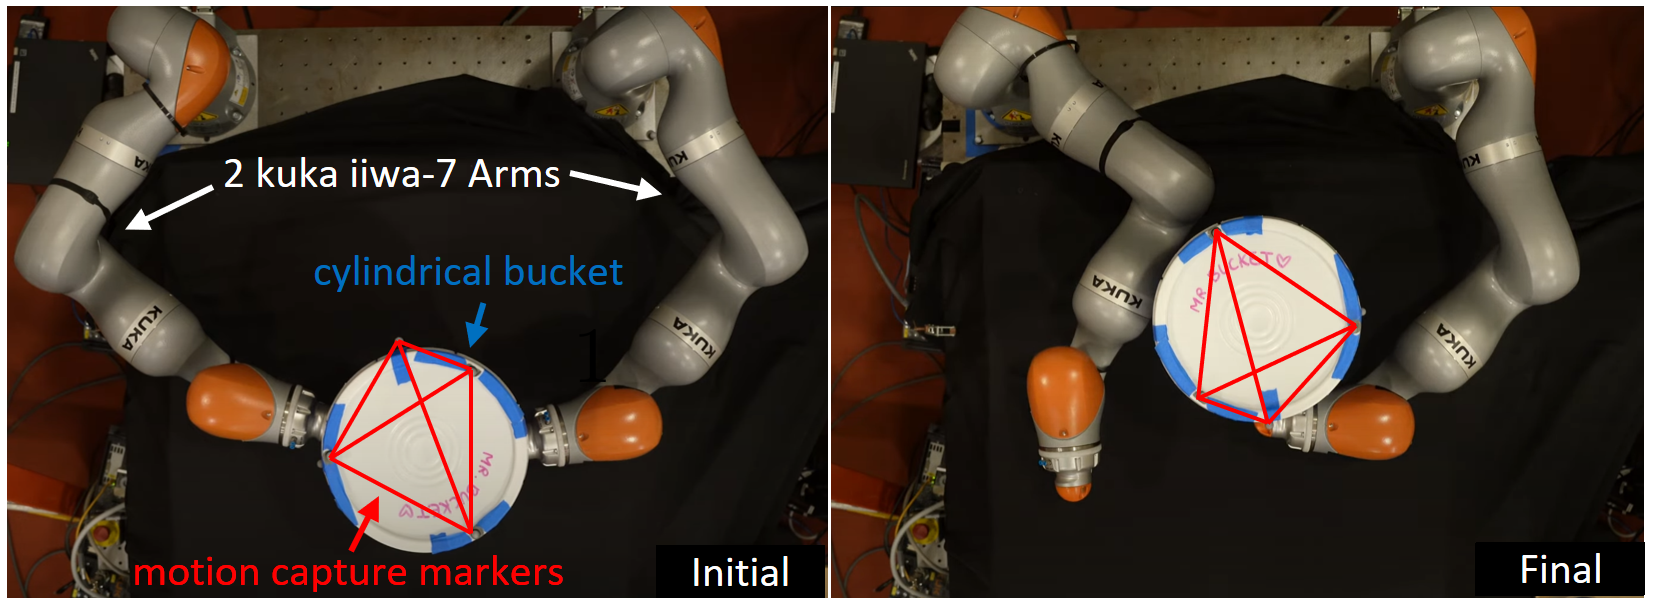
\includegraphics[width = 1.0\linewidth]{figures/03_contact_rich_planning/hardware_setup.png}
\caption{Hardware for the \code{IiwaBimanual} setup, where the goal is to rotate the bucket by $180^\circ$. The left and right pictures correspond to the initial state and the final state after the open-loop plan execution. The lines between motion capture markers are connected to illustrate the change of pose in the bucket. Readers are encouraged to watch the accompanying video for the full execution.} 
\label{fig:hardware}
\end{figure}


\subsection{Results \& Discussion}
We plot the results of our experiments in Fig.\ref{fig:sim_to_real}. While 2D systems such as \code{PlanarPushing}, \code{PlanarHand}, and \code{IiwaBimanual} display low error and good sim2real transfer, 3D systems such as \code{AllegroHand}, \code{AllegroPlate}, \code{AllegroPen} and \code{AllegroDoor} show larger error. To better understand the discrepancy of sim2real performance on different systems, we visualized trajectories from all systems by overlaying $\qurealp$ on top of $\qsimp$ (some of these visualizations are shown in the accompanying video). 

\begin{figure*}[thpb]
\centering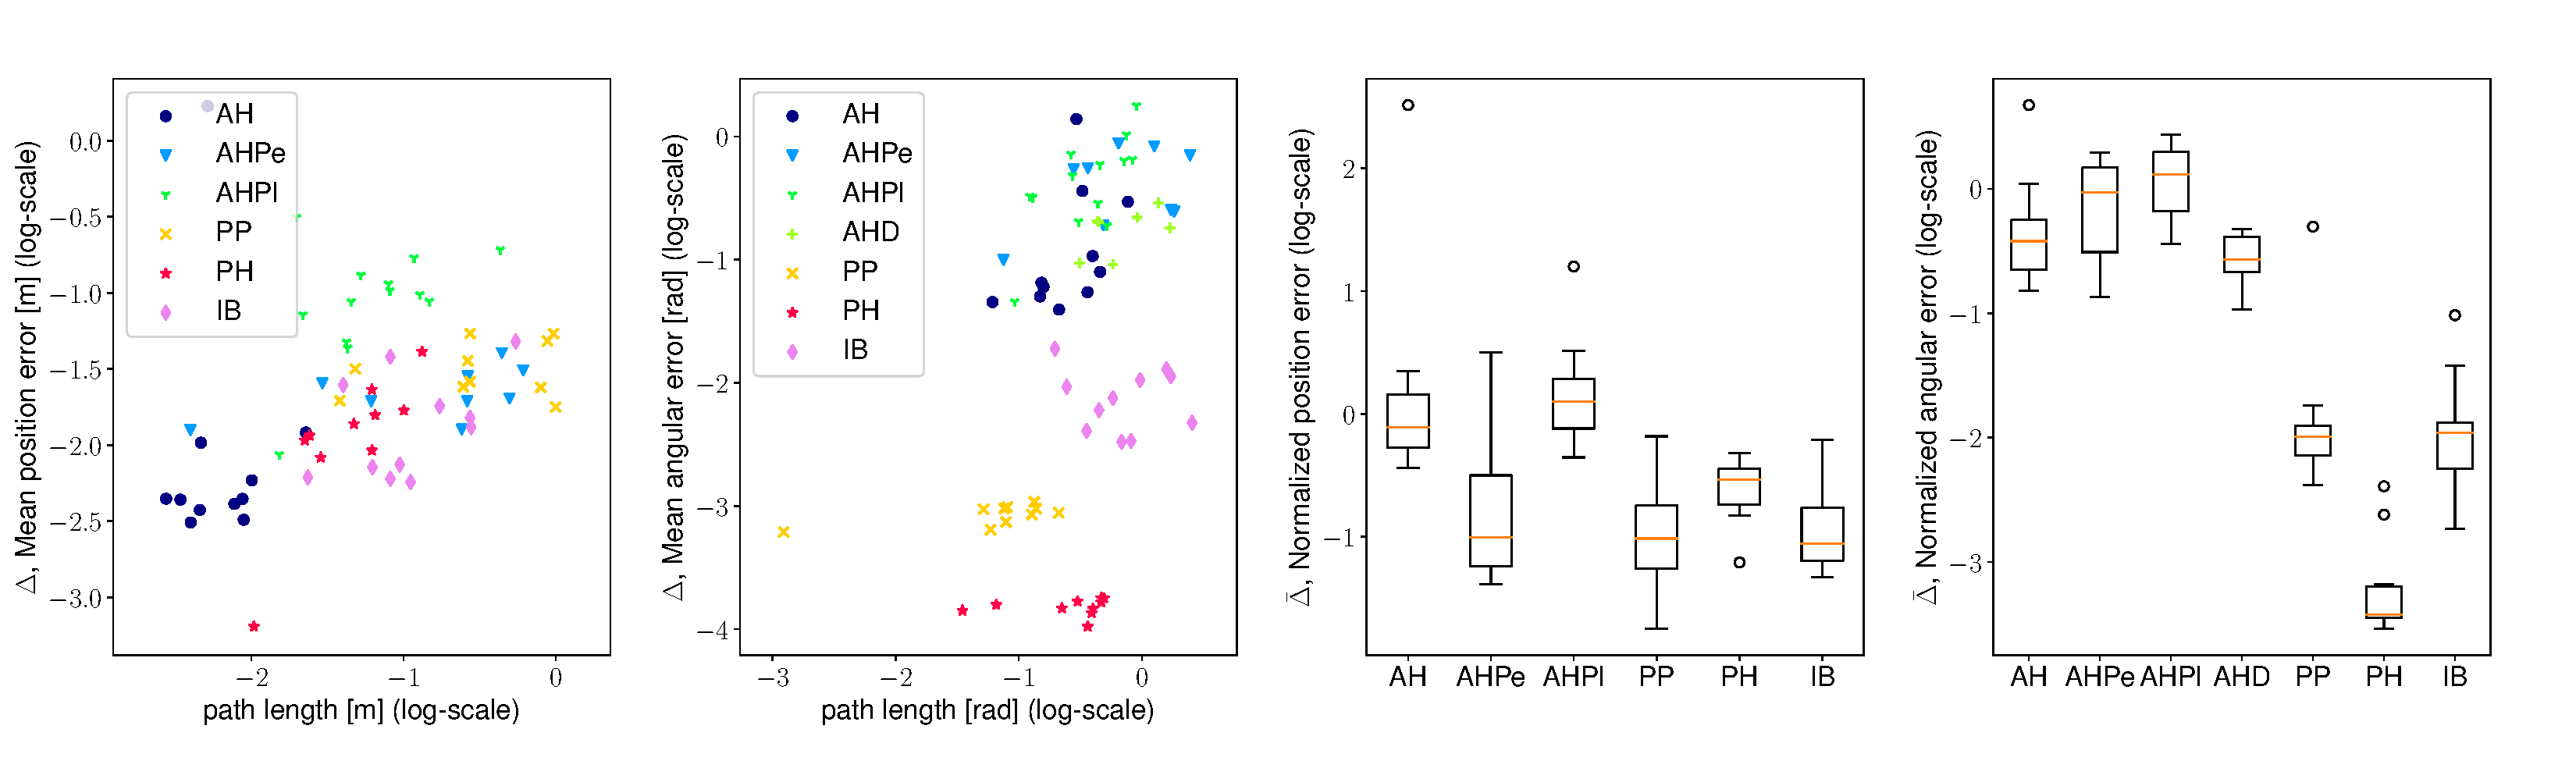
\includegraphics[width = 1.0\linewidth]{figures/03_contact_rich_planning/sim_to_real.pdf}
\caption{Plots for sim2real performance of our CQDC dynamics, evaluated on the plans of Sec.\ref{sec:rrt_results}. \textbf{First Two Columns}: Scatter plot of mean error $\Delta$ vs. path length for position (first column) and orientation (second column). Each dot in the plot represents one segment trajectory. \textbf{Last Two Columns}: Box plot for the normalized error $\bar{\Delta}$ for positions (third column) and orientation (fourth column). Note that the mean in orange corresponds to the slope of the graph in the first two columns. Finally, we note that the \code{AllegroHandDoor} (AHD) example only consists of orientation, and has no position plot. Readers are highly encouraged to watch the accompanying video for the qualitative behavior of the actual segment trajectories in this plot.}
\label{fig:sim_to_real}
\end{figure*}

From the video, it is clear that on \emph{all} systems, there exists a persistent \emph{phase} difference between $\qurealp$ and $\qusimp$: $\qurealp$ tends to lag $\qusimp$ when the robot accelerates, and lead when the robot decelerates. This is not surprising, as the CQDC dynamics that generates $\qusimp$ is inherently a first-order system, whereas $\qurealp$ is generated from second-order dynamics. 
On trajectory segments with good sim2real performance, the phase gap only results in harmless oscillations of $\qurealp$ around $\qusimp$. In these cases, we believe that the good sim2real performance validates our contact model. 
However, the phase gap can have more serious consequences, which we will discuss next.


\subsubsection{Violation of Quasi-static Assumption} 
The quasi-static assumption implies that objects are quickly stopped by damping when they are not ``pushed around'' by the robot. This is true on 2D systems, as the friction patch between the object and its supporting surface is persistent and always provides enough damping to bring the object to still. 

However, the necessary damping to uphold the quasi-static assumption does not always exist on 3D systems. For instance, in \code{AllegroHand} and \code{AllegroHandPen}, the point contact between the object and the palm provides very little damping. Most of the damping comes from the finger joints when the fingers are opposing the object's motion. Therefore, when the grasp on the object ``leaves an opening'', the object can roll quite far from the planned trajectory or even off the palm. 

\subsubsection{Missed Contacts}
Due to the non-smooth nature of contact dynamics, small discrepancies in object trajectory caused by the phase gap can lead to the robot completely missing contacts with the object. For example, we observed that in \code{AllegroHandPlate} or \code{AllegroHandDoor}, some grasps that were valid under the CQDC dynamics no longer succeeded in holding the object in place in Drake. The consequence of these failed grasps is that plates are dropped on the table in \code{AllegroHandPlate}, and door handles are missed in \code{AllegroHandDoor}.


\subsubsection{Necessity of Stabilization \& Robustification}
These results tell us that the plan suggested by the CQDC dynamics might give a high-level direction, but its open-loop execution may not succeed under second-order dynamics with high velocities and low amount of damping. We believe that tracking this high-level plan requires low-level feedback controllers that can stabilize to the plan, and actively enforce the closed-loop system to be quasi-static. We also believe that the high-level planer can benefit from robustness objectives such as encouraging grasps that are considered good under classical grasping metrics. Such grasps will increase the control authority of the robot over the object, thereby providing sufficient damping and decreasing the chances of dropping the object. We leave these as promising directions for future work. 